% Preamble %%%%%%%%%%%%%%%%%%%%%%%%%%%%%%%%%%%%%%%%%%%%%%%
\documentclass{thesis}
%%%%%%%%%%%%%%%%%%%%%%%%%%%%%%%%%%%%%%%%%%%%%%%%%%%%%%%%%%
%\usepackage{setspace}
%\usepackage[xindy]{glossaries}
%\newglossarystyle{customstyle}{%
%% put the glossary in the itemize environment:
%\renewenvironment{theglossary}{}{}%
%% have nothing after \begin{theglossary}:
%\renewcommand*{\glossaryheader}{}%
%% have nothing between glossary groups:
%\renewcommand*{\glsgroupheading}[1]{}%
%\renewcommand*{\glsgroupskip}{}%
%% set how each entry should appear:
%\renewcommand*{\glossaryentryfield}[5]{%
%%\item[] % bullet point
%\glstarget{##1}{##2}% the entry name
%\dotfill% the symbol in brackets
%\space ##3 \\% the number list in square brackets
%}%
%% set how sub-entries appear:
%\renewcommand*{\glossarysubentryfield}[6]{%
%\glossaryentryfield{##2}{##3}{##4}{##5}{##6}}%
%}
%\makeglossaries
%\glossarystyle{customstyle}
%\def\glossaryname{واژه نامه}
%\newglossaryentry{گروه}{name=گروه,
%description={Group }}
%\newglossaryentry{چنبره}{name=چنبره,
%description={Torus }}
%\newglossaryentry{پردازشگر}{name=پردازشگر,
%description={Processor }}
%\newglossaryentry{کلاف}{name=کلاف,
%description={Bundle }}
%\newglossaryentry{شما}{name=شما,
%description={Scheme }}
%\newglossaryentry{رایانه}{name=رایانه,
%description={Computer }}
%\newglossaryentry{موسیقی}{name=موسیقی,
%description={Music }}
%\newglossaryentry{شعر}{name=شعر,
%description={Poem }}
%\newglossaryentry{زی‌پرشین}{name=زی‌پرشین,
%description={\XePersian }}
%\newglossaryentry{واژه‌نامه}{name=واژه‌نامه,
%description={Glossary }}
%\newglossaryentry{آنتن}{name=آنتن,
%description={Antenna }}
%%%%%%%%%%%%%%%%%%%%%%%%%%%%%%%%%%%%%%%%%%%%%%%%%%%%%%%%%%
\usepackage{rotating}
\usepackage{tikz}
\usepackage[colorlinks=true]{hyperref}
\usepackage{hyperref}
\hypersetup{
  linkcolor  = black,
  citecolor  = black,
  urlcolor   = black,
  colorlinks = true,
}
\usepackage{amssymb}
\usepackage{xepersian}
\settextfont[Scale=1]{XBNiloofar}
% Title page %%%%%%%%%%%%%%%%%%%%%%%%%%%%%%%%%%%%%%%%%%%%%
\begin{document}
\logo{
\includegraphics{logo}}
\date{
۴ تیر ۱۳۹۶
}
\title{
تحلیلی بر عملکرد حافظه مشترک تحت بارهای کاری چند منظوره در پردازنده‌های گرافیکی
}
\author{
پارسوآ خورسند رحیم‌زاده
}
\university{%
دانشگاه صنعتی شریف
\\
دانشکده مهندسی کامپیوتر
}
\subject{%
مهندسی نرم‌افزار
}
\supervisor{
دکتر حمید سربازی آزاد
}
\frontmatter \makethesistitle \pagestyle{empty} \baselineskip1.2\baselineskip
% Abstract %%%%%%%%%%%%%%%%%%%%%%%%%%%%%%%%%%%%%%%%%%%%%%%
\begin{abstract}
{%
پردازنده‌های گرافیکی عام‌منظوره، حافظه مشترک، کارایی، زمان دسترسی،
فرکانس ، موازات سطح ریسمان
}
{%
در پردازنده‌های گرافیکی روی هر چند‌پردازنده جریانی
%\newglossaryentry{sm}{
%name=چند‌پردازنده جریانی,
%description={Streaming Multiprocessor}
%}
یک واحد حافظه اختصاصی برای نگهداری داده‌های مربوط به فضای آدرس‌دهی مشترک 
%\newglossaryentry{sharedaddressspace}{
%name=فضای‌آدرس‌دهی مشترک,
%description={Shared Address Space}
%}
ریسمان‌های در حال اجرا تعبیه شده‌است. فضای این حافظه به بلوک‌های هر چندپردازنده
به
طور
جداگانه تخصیص می‌یابد و میان ریسمان‌های
%\newglossaryentry{thread}{
%name=ریسمان,
%description={Thread}
%}
 هر بلوک به طور مشترک استفاده می‌شود.

حافظه مشترک
%\newglossaryentry{sharedmemory}{
%name=حافظه مشترک,
%description={Shared Memory}
%}
 به برنامه‌نویس اجازه می‌دهد تا اطلاعات مورد نیاز برای اجرای هر بلوک از
ریسه‌های برنامه را روی چندپردازنده‌ جریانی شامل آن‌ها ذخیره کند. حافظه مشترک به
دلیل ظرفیت و در نتیجه مساحت کم و نیز قرار گرفتن روی تراشه چند‌پردازنده زمان
دسترسی بسیار پایینی (در حد چند کلاک) دارد. به این ترتیب برنامه‌نویس می‌تواند
بخشی از داده را که احتمال می‌دهد قرار است در باز زمانی فعلی با نرخ بالا مورد
دسترسی قرار گیرد را روی این حافظه بارگذاری
%\newglossaryentry{upload}{
%name=بارگذاری,
%description={Upload}
%}
  کند تا دسترسی به آن با سربار کم امکان‌پذیر باشد. 
  
  
  در نسل‌های اولیه پردازنده‌های گرافیکی، حافظه‌مشترک به عنوان راه‌حلی برای
مدیریت پیچیدگی‌های ناشی از زمان دسترسی غیر‌قابل پیش‌بینی حافظه‌ اصلی مورد
پیاده‌سازی قرار گرفت. چنین رویکردی در کاربرد‌های گرافیکی که نیاز به تضمین نرخ
فریم
%\newglossaryentry{framerate}{
%name=نرخ فریم,
%description={Frame Rate}
%}
ثابتی وجود دارد از توجیه‌پذیری بالایی برخوردار است.

در ادامه نتایج تحلیل روی عملکرد و میزان کاربرد حافظه مشترک در بارهای کاری
%\newglossaryentry{workload}{
%name=بار کاری,
%description={Workload}
%}
محاسباتی ارائه می‌شود و در نهایت راهکار‌هایی برای بهبود کارایی 
%\newglossaryentry{performance}{
%name=کارایی,
%description={Performance}
%}
این مدل حافظه پیشنهاد می‌گردد
.
}
\end{abstract}
% Appendix %%%%%%%%%%%%%%%%%%%%%%%%%%%%%%%%%%%%%%%%%%%%%%%
\pagestyle{plain} \pagenumbering{tartibi}
\tableofcontents
\listoffigures
\cleardoublepage
% Introduction %%%%%%%%%%%%%%%%%%%%%%%%%%%%%%%%%%%%%%%%%%%
\mainmatter \pagestyle{headings}\baselineskip1.1\baselineskip

\chapter{%
مقدمه
}

بر اساس قانون مور
\LTRfootnote{
Moore's Law
}
چگالی ترانزیستور‌های تراشه‌های نیمه‌رسانا
\LTRfootnote{
Semiconductor
}
پس از گذشته به طور تقریبی هر هجدهماه، دو‌ برابر می‌شود. در نتیجه می‌توان گفت که
پردازنده‌ها کوچکتر‌، چگال‌تر و قدرتمند‌تر می‌شوند. بر اساس این قانون حداکثر
فرکانس‌ کاری پردازنده‌ها نیز قابل افزایش به نظر می‌رسد. اما به دلایل گوناگون
روند افزایش  فرکانس کاری پردازنده‌ها در سال‌های اخیر با کندی مواجه شده است.
با ادامه روند افزایش فرکانس پردازنده‌ها، پیش‌بینی می‌شد که تا حوالی سال ۲۰۰۵
میلادی چگالی توان تراشه‌ها به سطح راکتور‌های هسته‌ای برسد.

\begin{figure}[h]
\centering
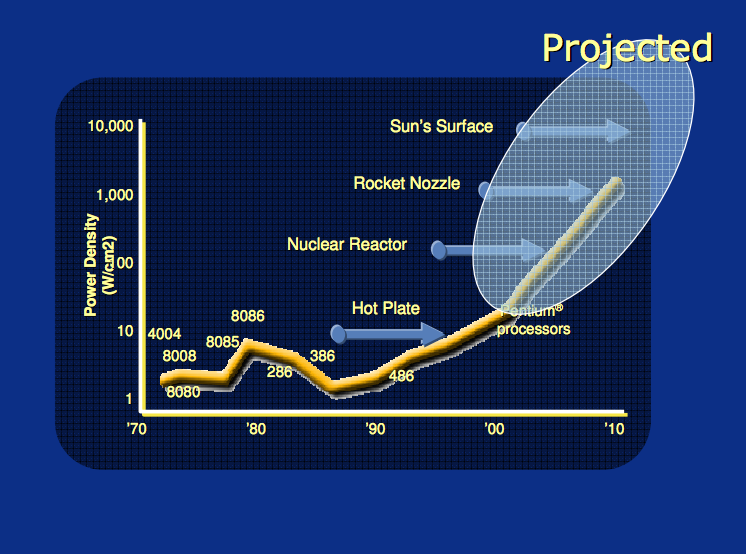
\includegraphics[width=\textwidth]{./pics/1}
\caption{پیش‌بینی رشد چگالی توان پردازنده‌ها}
\end{figure}

\section{پردازنده‌های چندهسته‌ای}

علی‌رغم پیشرفت‌ چشمگیر قدرت محساباتی سخت‌افزار‌ها و نیز نزدیک‌ شدن به موانع
عملی و فیزیکی برای افزایش فرکانس‌کاری آن‌ها، نیاز به بهبود عملکرد 
\LTRfootnote{Performance}
تراشه‌ها برای پشتیبانی از نیازمندی‌های جدید نرم‌افزار (به طور خاص رابط کاربری
گرافیکی) و نیز انجام‌ها پردازش رو مجموعه‌داده‌های
\LTRfootnote{Dataset}
 گسترده احساس می‌شد. 
در حدود سال ۲۰۰۰ میلادی اینتل
با معرفی پردازنده‌های با معماری
NetBurst
انتظار دستیابی به فرکانس کاری
\lr{10Ghz}
را داشت اما در عمل به علت مشکلات گرما و توان مصرفی عملیات این چیپ‌ها فرکانس‌های
بالای
\lr{4Ghz}
بدون استفاده از سیستم‌های خنک‌کننده بزرگ و پیچیده
(معمولا مبتنی بر آب)
امکان‌پذیر نبود.

 در این میان ایده
  پردازنده‌های چندهسته‌ای به عنوان راه‌حلی
برای افزایش کارایی ارائه شد. با توجه به اینکه در این فرکانس کاری پردازنده
افزایش نمیابد، پارامتر‌های توان مصرفی و در نتیجه چگالی توان نیز تغییر شگرفی
نمی‌کنند ولی چنانچه محسابات را بتوان به قسمت‌هایی با قابلیت موازی‌سازی تقسیم
کرد می‌توان زمان اجرا را به طور قابل توجهی کاهش داد. میزان 
ایده‌آل
بهبود عملکرد محاسبه
در این حالت از قانون امدال
\LTRfootnote{Amdahl's law}
پیروی می‌کند.

 لازم به ذکر است که تا قبل از ظهور پردازنده‌های چندهسته‌ای با 
تعریف امروزی گاها
از
چند پردازنده‌ی مرکزی مستقل برای انجام محاسبت استفاده می‌شد.  در این معماری هر
پردازنده عملا یک چیپ جداگانه بود که به واسطه یک باس
\LTRfootnote{Bus}
مشترک به مادربورد و حافظه اصلی متصل می‌شد. این استقلال فیزیکی پردازنده‌ها
مشکلات مختلفی ایجاد می‌کرد که در معماری‌های جدیدتر با قراردادن چند هسته
\LTRfootnote{Core}
 پردازشی
داخل یک تراشه 
تا حدی برطرف شده است.

\section{
پردازنده‌های گرافیکی
}

تاریخچه پردازنده‌های گرافیکی به حدود سال‌های دهه ۷۰ میلادی بازمی‌گردد، زمانی که
واحد‌های سخت‌افزاری جداگانه برای بهبود عملکرد رایانه در اجرای باز‌ی‌ها استفاده
می‌شد. نسخه‌های اولیه چنین پردازنده‌هایی چیزی عملا گسترش جزیی معماری
پردازنده‌های
برداری
\LTRfootnote{Vector Processor}
برای کاربرد‌های گرافیکی بودند. در چنین پردازنده‌هایی که به طور خاص برای پردازش
سیگنال
و
داده‌های
در
قالب ماتریس و آرایه طراحی شده بودند، تعداد زیادی واحد ریاضیاتی
\LTRfootnote{Arithmetic Logic Unit}
 به طور
همزمان دستورات یکسانی را روی قسمت‌های مختلف داده ورودی اجرا می‌کردند. این
رویکرد که به اصطلاح مدل
\textit{دستور واحد و داده‌های متفاوت}
\LTRfootnote{Single Instruction, Multiple Data (SIMD)}
نامیده می‌شود
به طور خاص در محاسبات جبر خطی
\LTRfootnote{Linear Algebra}
سودمند است.

پردازنده‌های گرافیکی در ابتدا سخت‌افزار‌هایی با عملکرد ثابت
\LTRfootnote{Fixed-Function}
بودند و امکان برنامه‌پدیری 
\LTRfootnote{Programmability}
نداشتند.
با افزایش قدرت پردازنده‌های گرافیکی طی نسل‌های متمادی و آشکار شدن پتانسیل این
روش پردازش برای کاربرد‌هایی خارج از حوزه گرافیک و بازی‌های رایانه‌ای، به مرور
زمان قابلیت برنامه‌پذیری نسبی به این سخت‌افزار‌ها اضافه شد و امروزه واسط‌های
نرم‌افزاری سطح بالای قدرتمندی مانند کودا
\LTRfootnote{CUDA: Compute Unified Device Architecture}
 توسعه داده
توسط شرکت
Nvidia
و
OpenCL
برای منظور پیاده‌سازی برنامه‌های موازی عام‌منظوره روی این تراشه‌ها 
در دسترس هستند.

یک پردازنده گرافیکی به طور معمول متشکل است از تعدادی چند‌پردازنده
\LTRfootnote{Multiprocessor}
که به صورت موازی دستورات (نه لزوما یکسان) را اجرا می‌کنند. به عنوان مثال
پردازنده گرافیکی
\lr{Nvidia Tesla K40}
بر پایه معماری
\lr{Kepler}
از ۱۵ چند‌پردازنده‌ جریانی
\LTRfootnote{Streaming Multiprocessor (SM)}
هر کدام با 
۱۹۲
هسته پردازشی عدد طبیعی
\LTRfootnote{Integer}
، ۶۴ هسته پردازشی عدد ممیزدار
\LTRfootnote{Floating Point}
 و ۳۲ واحد انتقال داده
\LTRfootnote{Load/Store Unit}
تشکیل یافته است.
این هسته‌ها به ۱۲ مجموعه 
\textit{دستور واحد و داده‌های متفاوت}
تقسیم می‌شود که هریک می‌توانند به طور مستقل دستور
واحدی‌ را روی داده ورودی خود اجرا کند
.
همچنین هر
چند‌پردازنده‌ جریانی
دارای یک واحد حافظه مشترک
\LTRfootnote{Shared Memory}
میان تمام هسته‌های پردازشی خود است که برای ذخیره داده‌های مورد نیاز در پردازش
فعلی و عدم نیاز به بارگیری
\LTRfootnote{Fetch}
آن‌ها از حافظه اصلی  در حین اجرا استفاده می‌شود.

در چنین معماری که با نام
\textit{دستور واحد و ریسه‌های متعدد}
\LTRfootnote{Single Instruction, Multiple Threads (SIMT)}
بازاریابی می‌شود تعداد زیادی
ریسه
به طور همزمان روند‌های اجرایی متفاوتی را روی داده اعمال می‌کنند.
یک پردازنده گرافیکی با معماری کپلر می‌تواند
۲۸۸۰
ریسه را به صورت موازی اجرا کند.

\begin{figure}[h]
\centering
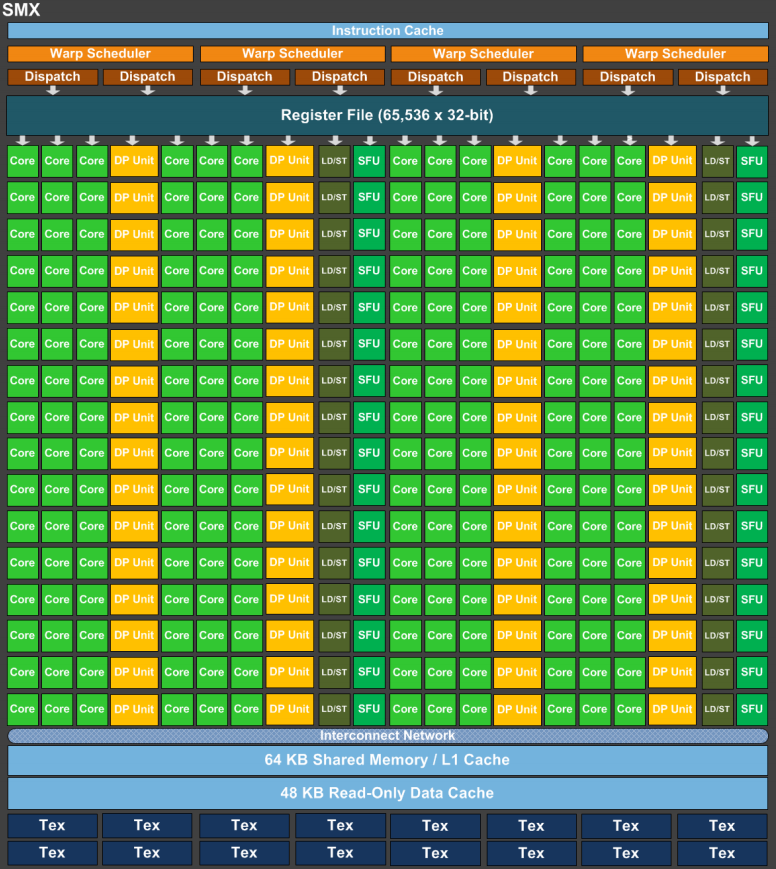
\includegraphics[width=0.7\textwidth]{./pics/2}
\caption{%
ساختار داخلی یک چندپردازنده جریانی در معماری
Kepler
}
\end{figure}

به لطف وجود چنین ظرفیت موازی‌سازی گسترده‌ای در پردازنده‌های گرافیکی زمان اجرای
محاسبات روی آن‌ها به شکل قابل توجهی کاهش می‌یابد. اما به دلایل مختلف 
مانند وابستگی‌داده‌ای بین دستورات، عدم قابلیت موازی‌سازی همه بخش‌های
پردازش، رفتار‌های مختلف
\LTRfootnote{Divergence}
 ریسه‌ها و در دستورات تصمیم‌گیری
\LTRfootnote{Decision Making}
و همچنین تاخیر‌های دسترسی به حافظه کارای پردازنده گرافیکی در شرایط واقعی بسیار
پایین‌تر از مقدار آن روی کاغذ است.

\section{ساختار پایان‌نامه}

در ادامه و پس از پایان مقدمه، در فصل دوم مفاهیم پایه‌ای در طراحی پردازنده‌های
چندهسته‌ای و به خصوص پردازنده‌های 
گرافیکی و به خصوص ساختاربندی حافظه در این تراشه‌ها را بررسی می‌کنیم. فصل سوم
مروری بر کارهای پیشین در موضوع پایان‌نامه خواهد بود. در فصل چهارم شهود و
انگیزه‌های اولیه برای این مطالعه را بررسی می‌کنم فصل پنجم را به معرفی
شبیه‌ساز و بررسی نتایج حاصل از شبیه‌سازی اختصاص می‌دهیم.
در
نهایت در فصل
ششم
به
جمع‌بندی و بررسی کارهای آتی می‌پردازیم.

% Chapter 2 %%%%%%%%%%%%%%%%%%%%%%%%%%%%%%%%%%%%%%%%%%%%%%

\chapter{
مفاهیم پایه‌
}

در این فصل ابتدا مروری کلی بر مفاهیم پردازنده‌های چند‌هسته‌ای و دلایل روی‌آوردن
به این پردازنده‌ها خواهیم داشت. در ادامه به بیان کلیاتی در مورد پردازنده‌های
گرافیکی و معماری و مدل برنامه‌سازی آن‌ها خواهیم پرداخت.

\section{
دلایل روی آوردن به پردازنده‌های چند‌هسته‌ای
}

زمانی که اندازه مشخصه
\LTRfootnote{Feature Size}
تزانزیستور‌ها با فاکتور
$k$
کاهش می‌یابد، به دلیل کوتاه‌تر شدن سیم‌ها و کاهش اندازه خازن در گیت‌ها
\LTRfootnote{Gate}
،
فرکانس کلاک
\LTRfootnote{Clock}
نیز با فاکتور
$k$
قابل افزایش است. همچنین تعداد ترانزیستور‌های موجود در واحد سطح با فاکتور
\lr{$x^2$}
و
اندازه قالب
\LTRfootnote{Die}
ترازیستور‌ها نیز با فاکتور
\lr{$k$}
قابل افزایش  می‌یابد. در چنین شرایطی قدرت پردازشی نیز به صورت تئوری با فاکتور
\lr{$k^4$}
افزایش  می‌یاد. هرچند در عمل به دلیل مواردی مانن توازی پنهان
\LTRfootnote{$Hidden Parallelism$}
 یا رفتار غیرقابل
پیش‌بینی حافظه نهان
\lr{$x^3$}
این فاکتور به طور عملی در مرتبه
\lr{$x^3$}
افزایش می‌یابد. به این نسبت‌ها قانون دانار گفته می‌شود
\LTRfootnote{Dannar Scaling (MOSFET Scaling)}
.
با این اوصاف به نظر می‌رسد که با معرفی هر نسل جدید پردازنده‌ها با اندازه مشخه
کوچکتر باید شاهد بهبود شگرف در عملکرد نرم‌افزارها باشیم. اما در عمل این رشد با
موانعی روبه‌روست که در ادامه به آن‌ها می‌پردازیم.

\begin{figure}[h]
\centering
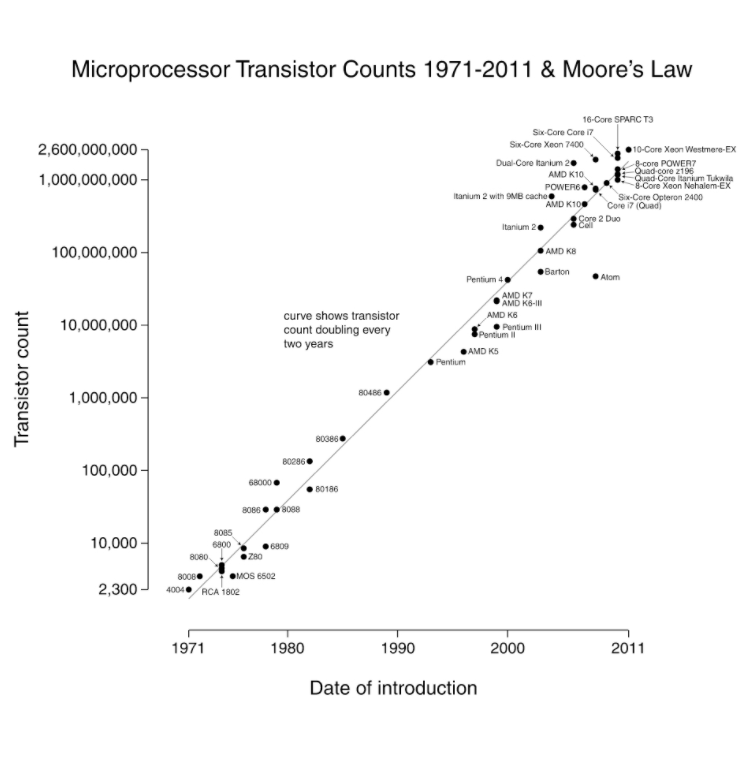
\includegraphics[width=\textwidth]{./pics/5}
\caption{تبعیت رشد تعداد ترانزیستور‌ها از قانون مور}
\label{moorelaw}
\end{figure}

\subsection{
چگالی توان
}

چگالی توان
\LTRfootnote{Power}
 به شکل میزان توان (نرخ انتقال انرژی) بر واحد حجم تعریف می‌شود. میزان
مصرف توان در تراشه‌ها به نرخ تغییر وضعیت گیت‌ها، یعنی نرخی که در آن 
خروجی یک گیت از صفر به یک تغییر می‌کند، بستگی‌دارد.
به
این
دلیل
به
اصطلاح گفته می‌شود که تراشه‌ها نرخ توان مصرفی پویا دارند.
با توجه به توضیح فوق انتظار می‌رود که نرخ توان مصرفی با افزایش فرکانس به طور
خطی افزایش پیدا کند. با توجه به افزایش نمایی فرکان پردازنده‌ها در سال‌های
پایانی دهه ۹۰ و اوایل قرن ۲۱ام، انتظار می‌رفت چگالی توان پردازنده‌ها در صورت
حفظ این نرخ رشد تا سال ۲۰۱۰ میلادی به ۱۰۰۰۰
وات بر سانتی‌متر مربع یعنی چیزی در حدود چگالی توان در سطح خورشید برسد. واضح است
که تراشه‌های نیمه رسانا در چنین وضعیتی تبخیر خواهند شد.

\subsection{
دیوار حافظه
}

به طور معمول هر دسترسی به حافظه اصلی
\LTRfootnote{Random Access Memory (RAM)}
در حدود صدها سیکل کلاک زمان می‌برد. به طور مثال پردازنده ممکن است برای اجرای
محاسبه‌ای که چند کلاک طول بکشد صدها کلاک منتظر دریافت داده و نوشتن مجدد آن در
حافظه بماند. به طور میانگین در سال‌های گذشته فرکانس حافظه هر 
شش سال دوبرابر می‌شد در حالی‌که که در تبیعت از قانون مور فرکانس پردازنده هر
دو سال دو برابر می‌شد. این تفاوت در نرخ رشد سبب ایجاد یک شکاف بزرگ میان عملکرد
پردازنده و حافظه می‌شود و حافظه را به گلوگاهی
\LTRfootnote{Bottleneck}
برای عملکرد سیستم تبدیل می‌کند و تاثیر افزایش فرکانس پردازنده را به شدت کاهش
می‌دهد. معماران سخت‌افزار با بهره‌گیری از ایده‌ها و روش‌های مختلف از جمله 
استفاده از چندین
لایه حافظه نهان و بهینه سازی‌هایی مانند 
\textit{%
بارگذاری با تاخیر
}
\LTRfootnote{Lazy Writeback}
و 
\textit{
کپی هنگام نوشتن
}
\LTRfootnote{Copy on Write}
سعی در مخفی کردن اثر سرعت حافظه از دید پردازنده دارند اما در نهایت مشکل همچنان
باقی است.
شکل
\ref{memorygap}
شکاف بین عملکرد پردازنده و حافظه اصلی را در سال‌های گذشته نشان می‌دهد.

\begin{figure}[h]
\centering
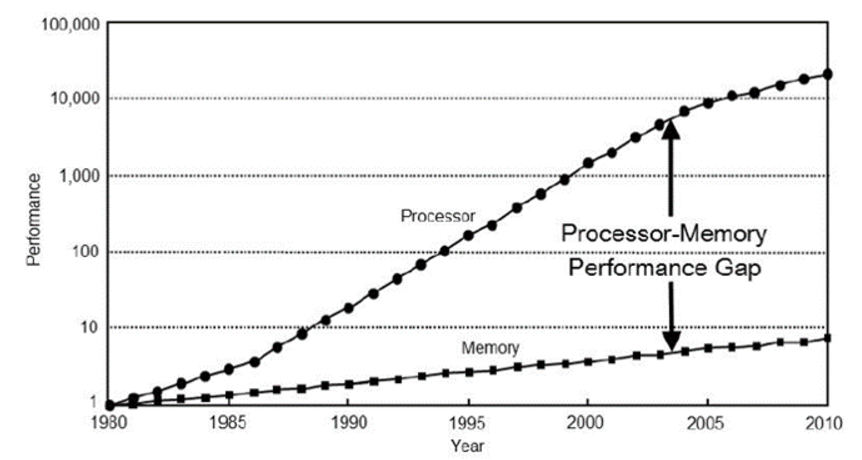
\includegraphics[width=\textwidth]{./pics/3}
\caption{شکاف بین عملکرد حافظه و پردازنده}
\label{memorygap}
\end{figure}

\begin{figure}[h]
\centering
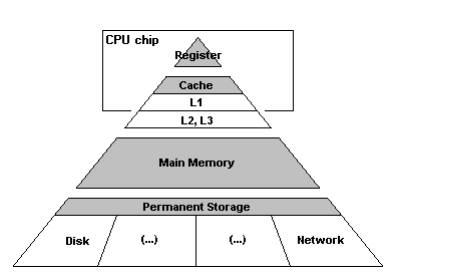
\includegraphics[width=\textwidth]{./pics/4}
\caption{سلسله مراتب حافظه در یک پردازنده امروزی}
\label{memoryhierarchy}
\end{figure}

\section{
پردازنده‌های چند‌هسته‌ای به عنوان یک راه‌حل
}

در زمانی که افزایش فرکانس پردازنده‌ها دیگر ممکن به نظر نمی‌رسد، مهندسان ایده
استفاده از چند پردازنده روی یک تراشه را برای بهبود عملکرد مطرح کردند. با توجه
به اینکه کارایی یک پردازنده با فرکانس کاری و تعداد هسته‌های آن متناسب است، با
افزایش تعداد هسته و ثابت نگه داشتن فرکانس می‌توانیم به عملکرد بهتری برسیم. با
پذیرفته شدن این معماری توسط تولید کنندگان مطرح مانند
Intel
و
AMD
از آن به بعد:

\begin{itemize}
\item 
چگالی ترانزیستو‌ر‌ها می‌تواند مانند قبل هر دو سال دو‌ برابر 
شود
\item
فرکانس پردازنده‌ها افزایش نمیابد (بعضا شاهد کاهش فرکانس برای ملاحظات توان مصرفی
هستیم)
\item
به جای دو برابر کردن فرکانس تمرکز روی دو برابر کردن تعداد هسته‌های پردازشی است
\end{itemize}


\section{
پردازنده‌های گرافیکی عام‌منظوره
}

به پردازنده‌های گرافیکی که قابلیت برنامه‌ریزی داشته باشد پردازنده گرافیکی
عام‌منظوره
\LTRfootnote{General Purpose Graphics Processing Unit}
گفته می‌شود. امروزه عمده کاربرد این پردازنده‌ها در محاسبات سنگین، شکستن رمز‌ها،
ارز‌های رمزنگاری‌شده
\LTRfootnote{Cryptocurrency}
و شبیه‌سازی‌های علمی است.

بر خلاف پردازنده‌های مرکزی که برای
اجرای سیستم عامل و
 سوییچ کردن
\LTRfootnote{Context Switching}
 بین تعداد زیادی پردازه
\LTRfootnote{Process}
اجرا و پنهان کردن تاخیر‌های حافظه برای حفظ پاسخگویی حداکثری طراحی شده‌اند،
پردازنده‌های گرافیکی با هدف حداکثر سرعت در محاسبات تولید می‌شوند و بسیاری از
پیچیدگی‌های داخلی پردازنده مرکزی را از معماری خود حذف می‌کنند. شکل
\ref{cpugpuperformancegap}
شکاف بین عملکرد این دو سخت‌افزار‌ را در محاسبات روی اعداد ممیز‌دار نشان می‌دهد.

\begin{figure}[h]
\centering
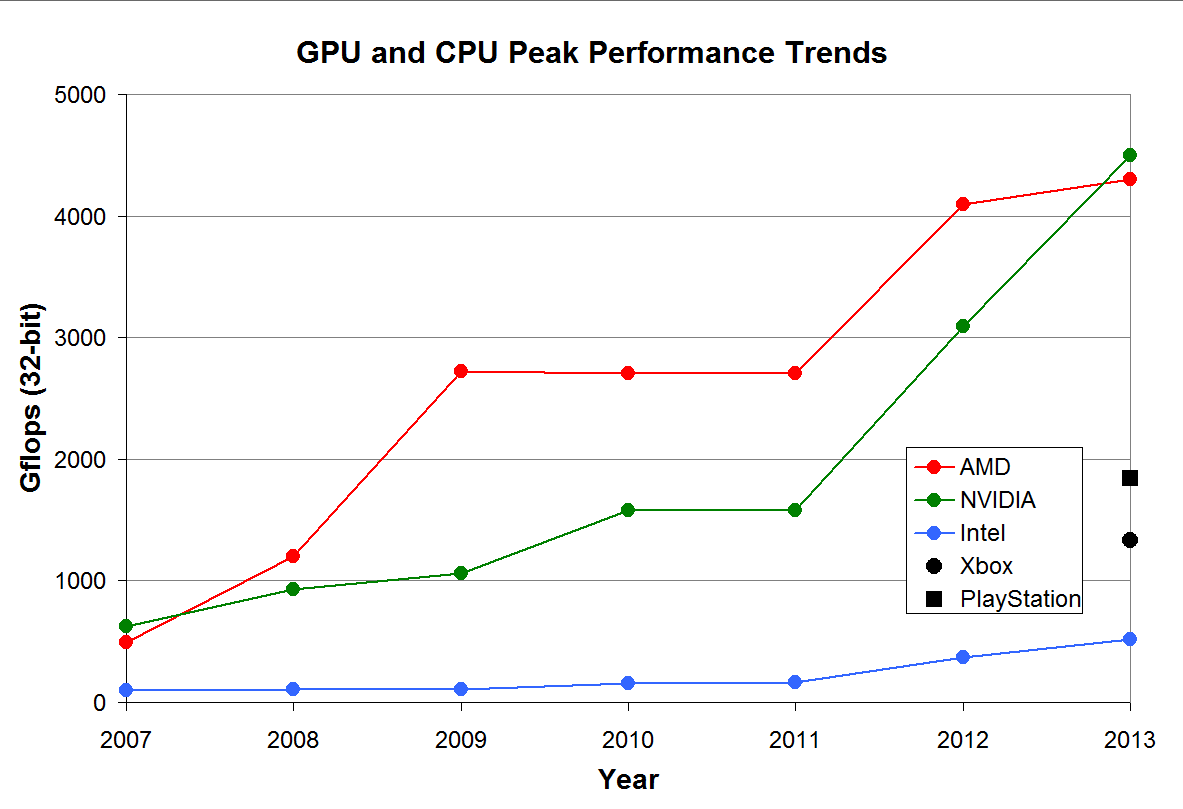
\includegraphics[width=\textwidth]{./pics/6}
\caption{شکاف بین عملکرد پردازنده مرکزی و پردازنده گرافیکی در محاسبات عددی}
\label{cpugpuperformancegap}
\end{figure}

\section{
استفاده از پردازنده گرافیکی برای مسائل عام‌منظوره
}

ایده استفاده از پردازنده‌های گرافیکی برای محاسبات عام منظوره به طور جدی از حدود سال ۲۰۰۳ مطرح بوده است. این پردازنده‌ها به دلیل موازات بالا همواره گزینه وسوسه‌کننده‌ای برای انواع محاسبات بوده‌اند. با توجه به طراحی پردازنده‌های گرافیکی به طور خاص برای اجرای بازی‌های سه‌بعدی، معماری دستور‌العمل
\LTRfootnote{Instruction Set Architecture (ISA)}
 آن‌ها نیز مبتنی بر کار با داده‌هایی راس‌های چند ضعلی‌ها (به طور خاص مثلث
\LTRfootnote{Triangulation}
)
، ماتریس‌های نگاشت در فضا و توصیف‌ 
shader
های گرافیکی بوده است. استفاده از چنین سخت‌افزاری برای محاسبات غیرگرافیکی نیازمند تعریف فضای مساله‌ هدف در قالب چنین ساختار‌های پایه‌ای و عملیات‌های جبر خطی روی آن‌ها بوده است. چنین فرآیندی علاوه بر پیچیدگی نیازمندی آشنایی دقیق با معماری داخلی سخت‌افزار بوده و عملا ریسک استفاده از این سخت‌افزار‌ها برای کاربرد‌های صنعتی را بسیار بالا می‌برد، در نتیجه استفاده از سخت‌افزار‌های گرافیکی برای محسابات عام‌منظوره به تحقیقات آکادمیک محدود باقی ماند.

برای اولین بار شرکت
Nvidia
با ارائه معماری
\lr{G80}
و رابط برنامه‌سازی
\LTRfootnote{Application Programming Interface (API)}
کودا
برای آن در اواخر سال ۲۰۰۶ پردازنده‌های گرافیکی قابل استفاده در محاسبات عام‌منظوره را معرفی کرد. از این تاریخ به بعد رشد بازار این پردازنده‌ها بسیار چشمگیر بوده و امروزه شاهد پردازنده‌های گرافیکی بهینه‌سازی شده برای کاربرد‌های خاص مانند شبکه‌های عصبی هستیم.

\begin{figure}[h]
\centering
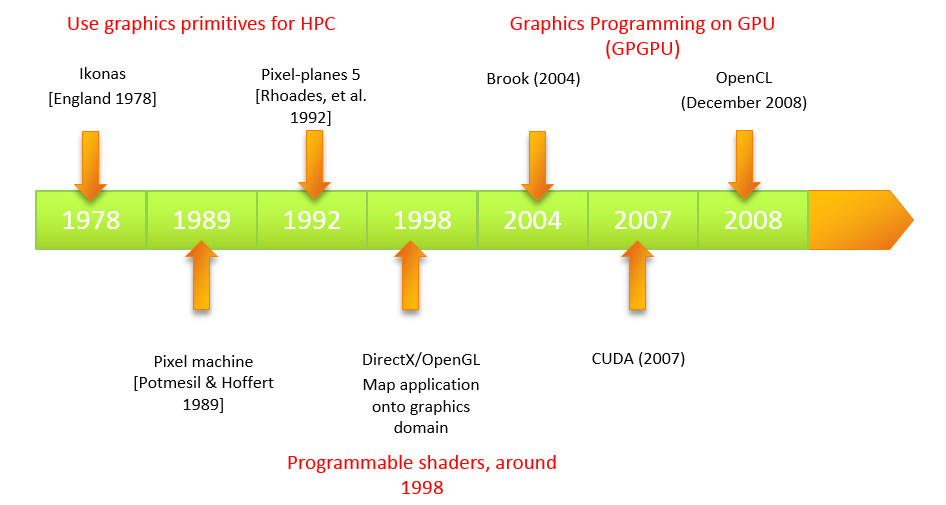
\includegraphics[width=\textwidth]{./pics/8}
\caption{
تاریخچه‌ای از استفاده از پردازنده‌های گرافیکی برای محاسبات عام‌منظوره
}
\end{figure}

\section{
معماری کودا
}

در قسمت به معرفی رابط برنامه‌سازی کودا و مفاهیم انتزاعی مطرح در آن برای انجام محاسبات چند‌منظوره روی پردازنده‌های گرافیکی می‌پردازیم.

\subsection{
کرنل
}

کودا محاسبات را در قالب فراخوانی پی‌دی‌پی مجموعه‌ای از کرنل‌ها
\LTRfootnote{Kernel}
 مدل‌سازی می‌کند
.
هر برنامه از دید کودا شامل دو قسمت است:

\begin{enumerate}
\item 
 بخش‌های ترتیبی که روی پردازنده مرکزی یا به اصطلاح میزبان
\LTRfoonote{Host}
اجرا می شود
\item
بخش‌های موازی که در میان بخش‌های ترتیبی روی پردازنده گرافیکی اجرا می‌شوند و پس از پایان هر قسمت از آن‌ها کنترل به پردازنده میزبان باز می‌گردد
\end{enumerate}

در این ساختار
به قسمتی از برنامه که به طور موازی رو پردازشگر گرافیکی اجرا می‌شود
کرنل می‌گویند.


\subsection{بلوک ریسه}

هر کرنل در قالب چند
بلوک ریسه
\LTRfootnote{Thread Block}
یا
آرایه ریسه‌ای هم‌محور
\LTRfootnote{Cooperative Thread Array}
رو سخت افزار اجرا می‌شود. یک سخت‌افزار کودا متشکل از تعدادی چندپردازنده جریانی است که هر کدام می‌توانند چندین بلوک ریسه را به طور هم‌زمان اجرا کنند. ریسه‌های هر بلوک از طریق حافظه مشترک روی چندپردازنده و سد‌های هم‌گام‌سازی
\LTRfootnote{Synchronization Barrier}
با هم در ارتباط هستند.

\subsection{توری}

توری 
\LTRfootnote{Grid}
مفهومی برای افزایش سطح استفاده از سخت‌افزار است. بلوک‌ها ریسه را می‌توان در قالب توری دسته‌بندی کرد، به این ترتیب چند کرنل و یا قسمت‌های مختلف یک کرنل می‌توانند در قالب توری‌های مختلف روی سخت‌افزار اجرا شوند. شکل
\ref{grid}
این سطح‌بندی را به روشنی نشان می‌دهد.

\begin{figure}[h]
\centering
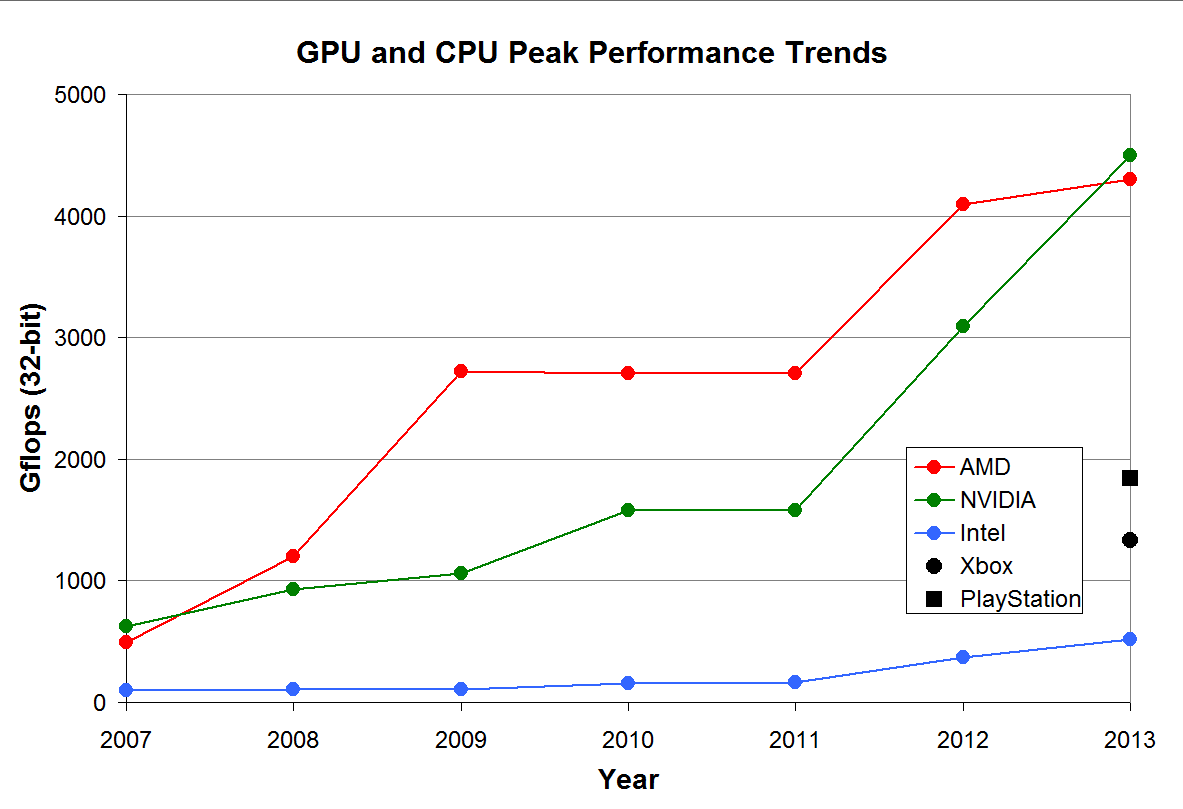
\includegraphics[width=\textwidth]{./pics/6}
\caption{
سطوح انتزاعی مدل‌سازی پردازش در معماری کودا
}
\label{grid}
\end{figure}

\subsection{تار}

چندپردازنده ریسه‌های هر بلوک را به گروه‌های ۳۲‌تایی به اسم تار
\LTRfootnote{Warp}
تقسیم می‌کند و سپس اجرای تار‌ها را روی منابع خود برنامه‌ریزی می‌کند. تمام ریسه‌های یک تار دستور یکسانی را اجرا می‌کنند. این کار اجازه می‌دهد تا در صورت کمبود منابع چند بلوک در قالب تارهای مستقل به طور هم‌زمان روی یک چندپردازنده اجرا شوند. شکل
\ref{warpschedule}
این مورد را نشان می‌دهد.

\begin{figure}[h]
\centering
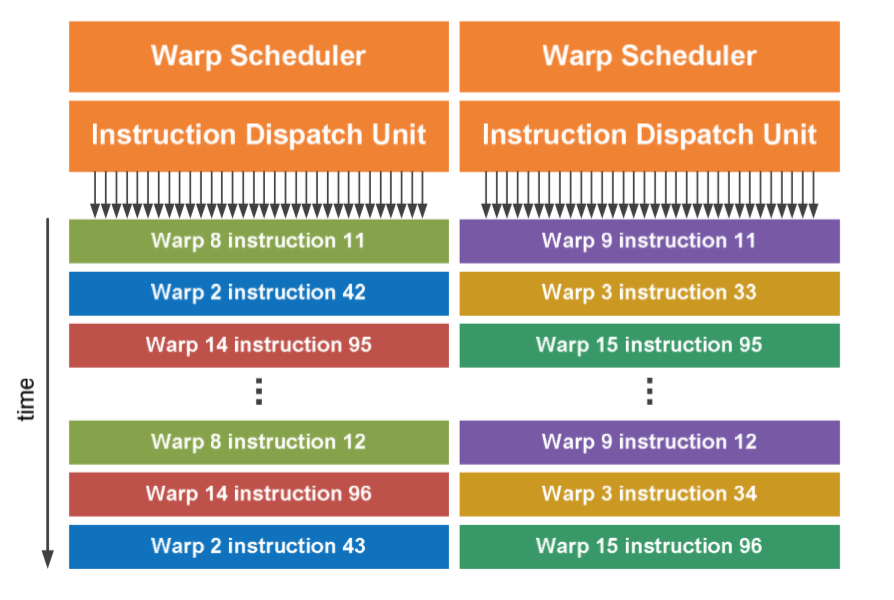
\includegraphics[width=\textwidth]{./pics/9}
\caption{%
اجرای هم‌زمان چند بلوک در قالب تار‌ روی یک چندپردازنده
}
\label{warpschedule}
\end{figure}

\subsection{ارتباط پردازنده گرافیکی با پردازنده میزبان}

ارتباط پردازنده گرافیکی با پردازنده میزبان از طریق واسط
\LTRfootnote{Interface}
\lr{PCI-Express}
انجام می‌شود. این واسط ارتباط بین دو تراشه را با پهنای باند حدود ۱۰ گیگابیت بر ثانیه برقرار می‌کند.

در فرآیند اجرای یک برنامه توسط کودا مراحل زیر انجام می‌شوند:
\begin{enumerate}
\item
داده‌های موجود در حافظه پردازنده مرکزی (از جمله کد کرنل) به حافظه پردازنده گرافیکی منتقل می‌شود
\item
تابع کرنل توسط پردازنده اصلی روی پردازنده گرافیکی فراخوانی می‌شود
\item
پس از پایان اجرای کرنل پردازنده گرافیکی کنترل را به پردازنده اصلی منتقل می‌کند
\item
در صورت نیاز نتایج محاسبه از حافظه پردازنده گرافیکی به پردازنده اصلی انتقال می‌یابد.
\end{enumerate}

\subsection{
سلسله مراتب حافظه در پردازنده گرافیکی
}

در پردازنده‌های گرافیمی به طور معمول ۵ لایه حافظه وجود دارد:

\begin{enumerate}
\item
حافظه سراسری
\LTRfootnote{Global Memory}
یا حافظه دستگاه
\item
حافظه بافت
\LTRfootnote{Texture}
\item
حافظه ثابت
\LTRfootnote{Constant}
\item
حافظه مشترک
\item
بانک ثبات
\LTRfootnote{Register Bank}
\end{enumerate}

حافظه سراسری یک حافظه دسترسی دلخواه
\LTRfootnote{Random Access Memory}
بوده و دارای حجم بالا و در نتیجه تاخیر دسترسی زیاد است. ارتباط پردازنده مرکزی و پردازنده گرافیکی از طریق
DMA
\LTRfootnote{Direct Memory Access}
روی درگاه
PCI
برقرار می‌شود. این حافظه توسط تمام چند پردازنده‌ها و ریسه‌ها قابل دسترسی است.

حافظه‌های بافت و ثابت نیز از نوع پویا هستند و از طریق پردازنده اصلی مقداردهی می‌شوند. این دو حافظه نیز  برای تمام ریسه‌ها قابل مشاهده هستند اما امکان نوشتن داخل آن فقط توسط پردازنده مرکزی وجود دارد (به همین دلیل به آن ثبت گفته می‌شود)
.

% Previous Works %%%%%%%%%%%%%%%%%%%%%%%%%%%%%%%%%%%%%%%%%
\chapter{
کارهای پیشین
}

در این فصل به طور اجمالی به بررسی مطالعات انجام شده روی موضوع این پایان‌نامه می‌پردازیم.

از آن‌جا که تاثیر حافظه مشترک در محدود کردن عملکرد پردازنده گرافیکی، به خصوص موازات سطح‌ ریشه و تعداد دستورالعمل در کلاک به اندازه‌ی سایر عوامل از جمله رجیستر ‌فایل، حافظه نهان و واگرایی پرش نیست، مطالعاتی محدودی روی این موضوع انجام شده است و مقالات کمی را می‌توان یافت که ایده‌های جدید در این زمینه مطرح کنند.

از جمله مقالات چند سال گذشته در مورد تاثیر حافظه مشترک و تاثیر آن عملکرد پردازنده‌های گرافیکی می‌توانی به
\cite{cite11}
,
\cite{cite12}
,
\cite{cite13}
و
\cite{cite14}
اشاره کرد. این مقالات بیشتر به مبحث عدم استفاده مناسب
\LTRfootnote{Underutilization}
از حافظه مشترک به علت تلاقی دسترسی به بانک‌های حافظه و وجود متغیر‌ها و داده‌های مشترک بین چند ریسه در آن اشاره کرد.

 رویکرد ما در این پایان‌نامه بررسی تاثیر حافظه مشترک در بارهای کاری محاسباتی عام‌منظوره و امکان جایگزینی این حافظه با راهکاری بهینه‌تر در  سخت‌افزارهای طراحی شده برای محاسبات سرعت بالا بوده است. چنین دیدی هرگز در مطالعات انجام‌ شده تا به امروز مورد توجه قرار نگرفته است، از این رو امیدواریم توانسته باشیم ایده‌های جدید وارد این حوزه کنیم.

% Motivation %%%%%%%%%%%%%%%%%%%%%%%%%%%%%%%%%%%%%%%%%%%%%
\chapter{
انگیزه و شهود
}

در این فصل ابتدا به بررسی وظایف حافظه مشترک و کاربرد‌های آن در پردازش‌های مختلف
می‌پردازیم و سپس روش‌های پیشنهادی خود را برای اندازه‌گیری عملکرد آن تحت بارهای
کاری علمی و نتایج به دست آمده را بررسی می‌کنیم.

در ادامه روشی برای بهبود عملکرد کلی تراشه گرافیک با تکیه بر تغییر معماری حافظه
مشترک پیشنهاد می‌دهیم و شهودی برای تاثیرگذار بودن این رویکرد ارائه می‌کنیم.

\section{
حافظه چرک‌نویس
}

حافظه چرک‌نویس 
\LTRfootnote{Scratchpad Memory}
به حافظه‌ای اطلاق می‌شود که نتایج میانی محاسبات را نگهداری می‌کند. 
scratchpad
معمولا نزدیک‌ترین واحد حافظه به
ALU
پس از رجیستر‌هاست و قادر به دسترسی مستقیم به حافظه اصلی
\LTRfootnote{Direct Memory Access (DMA)}
است. از آنجا که عمده نتایج میانی در محاسبات سنگین در پایان دور ریخته می‌شوند
استفاده از حافظه اصلی (و به تبع آن حافظه نهان) برای ذخیره‌سازی آن‌ها به علت
سرعت کم و نیز احتمال تاثیر منفی بر سایر دستورات در حال اجرا
(مصرف حافظه نهانی که می‌توانست به آن‌ها اختصاص پیدا کند) ضرورتی ندارد و در عوض
از یک حافظه سریع‌تر داخلی به این منظور استفاده می‌شود.

مزیت دیگر این واحد حافظه زمان دسترسی قابل پیش بینی به آن است، زیرا داده قبل از
رسیدن به پردازشگر از لایه‌های حافظه نهان عبور می‌کند و در زمان ثابتی قابل
دسترسی است.

\section{
حافظه مشترک
}

در پردازنده‌های مبتنی بر معماری کودا، به هر چندپردازنده‌ جریانی حافظه‌ای به
عنوان
\textit{%
حافظه مشترک
}
اختصاص داده می‌شود که عملا نقش همان چرک‌نویس را بازی می‌کند. برنامه‌نویس
می‌تواند از این حافظه برای ذخیره نتایج میانی و وضعیت فعلی پردازش و یا به عنوان
یک کپی سریع‌تر از حافظه اصلی استفاده کند. به عنوان مثال در معماری فرمی
%\LTRfootnote{Fermi}
هر چندپردازنده دارای یک واحد حافظه ۶۴ کیلوبایتی است که بستگی به نیاز می‌تواند
۱۶ یا ۴۸ کیلوبایت از آن را در ابتدای اجرای کرنل به عنوان حافظه مشترک استفاده
کند.

\section{
شبیه‌ساز
\lr{GPGPUSim}
}

\lr{GPGPUSim}
یک شبیه‌ساز نوشته شده به زبان
\lr{C++}
برای شبیه‌سازی عملکرد پردازنده‌های گرافیکی 
است. با اینکه تاکید اصلی در طراحی این شبیه‌ساز برای مطابقت آن با معماری
CUDA
بوده است، اما این شبیه‌ساز به صورت داخلی از مدل انتزاعل قابل  انعطافی استفاده
می‌کند
که می‌تواند در صورت لزوم برای شبیه‌سازی سخت‌افزار‌های دیگر تولید‌کنندگان هم
مورد استفاده قرار بگیرد.
این شبیه‌ساز نرخ دستور بر کلاک
\LTRfootnote{Instructions Per Clock (IPC)}
تقریبا یکسان
(با همبستگی حدود ۹۸ درصد با سخت‌افزار کودا) نشان می‌دهد و به از این جهت برای
سنجش عملکر پردازنده گرافیکی بسیار مناسب به نظر می‌رسد.
شکل
\ref{ipccorrelation}
این رفتار شبیه‌ساز را نشان می‌دهد
.
 بحث بیشتر در مورد جزییات داخلی این شبیه‌ساز خارج از
حوصله این نوشتار است.

\begin{figure}[h]
\centering
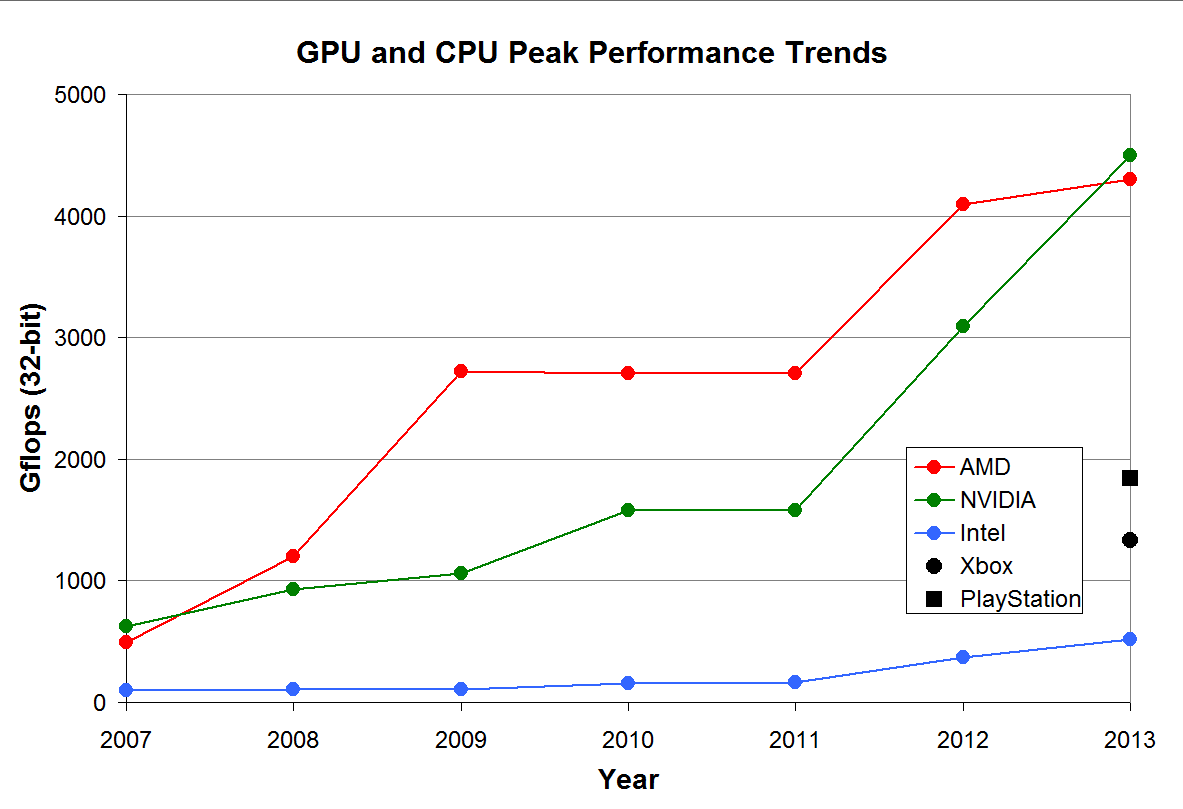
\includegraphics[width=\textwidth]{./pics/6}
\caption{همبستگی نرخ 
IPC
میان شبیه‌ساز و سخت‌افزار نسل
Fermi
}
\label{ipccorrelation}
\end{figure}

\subsection{
ثبت دسترسی‌ها به حافظه در شبیه‌ساز
}

برای ثبت دسترسی‌ها به حافظه لازم است تغییرات را داخل کد شبیه‌ساز اعمال کنیم.
فایل
\lr{\textit{instructions.cc}}
در پوشه
\lr{\textit{cuda-sim}}
شامل کد‌های مربوط به مدیریت دسترسی‌های حافظه است. روند اجرای تمام دستورات
خواندن
\LTRfootnote{Read}
و 
نوشتن
\LTRfootnote{Write}
به سطوح مختلف حافظه، چه به عنوان دستور مستقل و چه به عنوان بخشی از یک دستور
دیگر (مانند دسترسی به ثبات‌ها)
از توابع تعریف شده داخل این فایل می‌گذرد. موارد زیر را برای هر دسترسی ثبت
می‌کنیم:

\begin{itemize}
\item نوع دسترسی که می‌تواند
خواندن یا نوشتن باشد،
\item
آدرس مورد دسترسی
\item
تعداد بایت مورد دسترسی
\item
زمان دسترسی (شماره کلاک)
\item
شناسه کرنل 
\item
شناسه ریسه
\item
شناسه
CTA
\end{itemize}

\section{
بارهای کاری مورد استفاده
}

در طول این مطالعه برای بررسی عملکر حافظه مشترک از ۳ مجموعه بنچمارک
\LTRfootnote{Benchmark}
استفاده شده است:
\begin{enumerate}
\item 
مجموعه
بنچمارک
رودینیا
\LTRfootnote{Rodinia}
دانشگاه ویرجینا
\item
مجموعه بنچمارک
پاربویل
\LTRfootnote{Parboil}
دانشگاه
ایلینویز
\item
مجموعه بنچمارک
ISPASS
\end{enumerate}

این بنچمارک‌ها مجموعه‌ای از الگوریتم‌های رایج در حوزه‌های مختلف علمی و مهندسی
را پوشش می‌دهند که در جداول زیر به بررسی آن‌ها می‌پردازیم.

\begin{center}
\begin{table}[h!]
\begin{latin}
\begin{tabular}{|p{0.3\textwidth}|p{0.3\textwidth}|p{0.3\textwidth}|}
\hline
Benchmark & Summary & Application \\
\hline
BFS & Breadth-First Search & Graph Algorithms \\
\hline
CUTCP & Distance-Cutoff Coulombic Potential & Molecular Simulation \\
\hline
HISTO & Saturating Histogram & Statistics \\
\hline
LBM & Lattice-Boltzmann Method & Fluid Dynamics \\
\hline
MM & Dense Matrix-Matrix Multiply & Linear Algebra \\
\hline
MRI-GRIDDING & Magnteic Resonance Imaging - Gridding & Medical Imaging\\
\hline
MRI-Q & Magnetic Resonance Imaging - Q & Medical Imaging \\
\hline
SAD & Sum of Absolute Differences & MPEG video encoding \\
\hline
SPMV & Sparse-Matrix Dense-Vector Multiplication & Linear Algebra \\
\hline
SGEMM & Matrix-Matrix Multiplication & Linear Algebra \\
\hline
STENCIL & 3-D Stencil Operation & Graphics \\
\hline
TPACF & Two Point Angular Correlation Function & Atronomy \\
\hline
\end{tabular}
\end{latin}
\caption{%
\rl{%
گستره بنچمارک‌های موجود در پکیج پاربویل
}
}
\label{table:parboilbenchmarks}
\end{table}
\end{center}

\begin{center}
\begin{table}[h!]
\begin{latin}
\begin{tabular}{|p{0.3\textwidth}|p{0.3\textwidth}|p{0.3\textwidth}|}
\hline
Benchmark & Summary & Application \\
\hline
Kmeans & Dense Linear Algebra & Data Mining \\
\hline
Needleman-Wunsch (NW) & Dynamic Programming & Bioinformatics \\
\hline
HotSpot (HS) & Structured Grid & Physics Simulation \\
\hline
Back Propagation (BP) & Unstructured Grid & Pattern Recognition \\
\hline
SRAD & Structured Grid & Image Processing \\
\hline
Leukocyte Tracking (LC) & Structured Grid & Medical Imaging \\
\hline
Breadth-First Search (BFS) & Graph Traversal & Graph Algorithms \\
\hline
Stream Cluster (SC) & Dense Linear Algebra & Data Mining \\
\hline
MUMmer (MUM) & Graph Traversal & Bioinformatics \\
\hline
CFD Solver (CFD) & Unstructured Grid & Fluid Dynamics \\
\hline
LU Decomposition (LUD) & Dense Linear Algebra & Linear Algebra \\
\hline
Heart Wall Tracking (HW) & Structured Grid & Medical Imaging \\
\hline
\end{tabular}
\end{latin}
\caption{%
\rl{%
گستره بنچمارک‌های موجود در پکیج رودینیا
}
}
\label{table:parboilbenchmarks}
\end{table}
\end{center}


\begin{center}
\begin{table}[h!]
\begin{latin}
\begin{tabular}{|p{0.45\textwidth}|p{0.45\textwidth}|}
\hline
Benchmark & Summary \\
\hline
AES & Cryptography \\
\hline
Breadth-First Search (BFS) & Graph Traversal Algorithm \\
\hline
CP & N/A \\
\hline
DG & Discontinuous Galerkin Solvers \\
\hline
LPS & 3D Laplace Discretisation \\
\hline
LIB & N/A \\
\hline
MUM & High-Throughput Genome Sequence Alignment \\
\hline
NN & Neural Network \\
\hline
NQU & N-Queens Solver \\
\hline
RAY & Ray Tracing \\
\hline
STO & dDistributed storage systems \\
\hline
WP & Numerical Weather Prediction \\
\hline
\end{tabular}
\end{latin}
\caption{%
\rl{%
گستره بنچمارک‌های موجود در پکیج 
ISPASS
}
}
\label{table:ispassbenchmarks}
\end{table}
\end{center}

\subsection{%
دسترسی به حافظه مشترک در بارهای کاری مورد بررسی و انگیز اولیه
}

با اجرای شبیه‌ساز روی ۳۲ بار کار موجود در مجموعه سه بنچمارک مشاهده می‌شود که
تنها ۱۸ بار کاری در طی روند اجرای خود از حافظه مشترک استفاده می‌کنند.

\begin{center}
\begin{table}[h!]
\begin{latin}
\begin{tabular}{|p{0.45\textwidth}|p{0.45\textwidth}|}
\hline
Benchmark & Workloads \\
\hline
Parboil & BFS, CUTCP, HISTO, MRI-GRIDDING, SAD, SGEMM, STENCIL \\
\hline
Rodinia & HW, HS, LMD, NW, BP, PF \\
\hline
ISPASS & LPS, NQU, STO \\
\hline
\end{tabular}
\end{latin}
\caption{%
\rl{%
لیست بارهای کاری با دسترسی به حافظه مشترک
}
}
\label{table:sharedmemorybenchmarks}
\end{table}
\end{center}

با توجه به دامنه گسترده بارهای کاری مورد آزمون می‌توان ادعا کارد که این
بنچمارک‌ها طیف
کاملی
از کاربردهای عام منظوره رو پوشش می‌دهند. مشاهدات فوق انگیزه اولیه برای ادامه
این مطالعه را ایجاد می‌کند. حافظه مشترک در بسیاری از محاسبات عملا توسط
برنامه‌نویس مورد استفاده قرار نمی‌گیرد. با توجه به میزان قابل توجه حافظه مشترک
یافتن راه حلی برای استفاده بهینه از آن مستقل از نوع بارکاری در حال اجرا
می‌تواند عملکرد پردازنده را بهبود بخشد. برای  محسابه بهبود عملکرد پردازنده از
معیار
IPC
استفاده خواهیم.

تخصیص و آزاد‌سازی فضا روی حافظه مشترک توسط برنامه‌نویس و صریحا انجام می‌شود که
این امر می‌تواند پیچیدگی‌هایی را به همراه داشته باشد.
از زمان ظهور زبان‌های مدرن برنامه‌سازی، مدیریت حافظه به طور سنتی توسط کامپایلر
و یا محیط اجرا
\LTRfootnote{Runtime Environment}
انجام می‌شده و به خصوص در زبان‌هایی که بعد از 
\lr{C++}
وارد بازار شده‌اند، تدابیر مختلفی برای پنهان کردن جزییات روند مدیریت
حافظه از دید برنامه نویس اندیشیده شده است.
در داده‌ساختار‌های رایج مورد استفاده مانند آرایه، بردار، ماتریس، مجموعه بیت و
بعضا
لیست‌ها
\footnote{%
چنانچه پیاده‌سازی به شکل
آرایه پویا باشد
}
داده‌ها به شکل دنبال هم در حافظه ذخیره می‌شوند و از این رو در دسترسی به آن‌ها
 به طور طبیعی از
هم‌مکانی
\LTRfootnote{Locality}
بالایی برخوردار است که این مورد می‌تواند عملکرد حافظه نهان را به شکل قابل توجهی
افزایش دهد. به طور مثال در حوزه پردازش تصویر داده‌های اولیه معمولا مجموعه‌ای از
پیکسل‌ها هستند که به شکل طبیعی در قالب ماتریس ذخیره‌سازی می‌شوند و یا در
حوزه بایوانفورماتیک داده‌های مورد پردازش معمولا توالی‌های طولانی
ژنومی همراه با متاداده‌های اضافه‌شده به آن‌ها هستند. چنین داده ساختار‌های
ترتیبی‌ای
\LTRfootnote{Sequential}
به خوبی توسط سخت‌افزار مدیریت می‌شوند.

  به علاوه وجود یک حافظه مستقل از
RAM
و استفاده صریح از آن توسط برنامه‌نویس، ساختار کد را به معماری
سخت‌افزار و محدودیت‌ها آن وابسته می‌کند. همچنین با توجه به کارکرد مشخص 
حافظه مشترک،
چنانچه
ساختار
مساله نیازی به وجود آن نداشته باشد، تعداد قابل توجهی ترانزیستور در طی
روند اجرا بی ‌استفاده می‌مانند
و تنها توان مصرفی چیپ و گرمای تولید‌شده توسط آن‌را افزایش می‌دهند.

انگیزه اصلی ما در این پژوهش پیدا کردن راه حلی برای جایگزینی حافظه مشترک با
حافظه‌ای چند‌منظوره و تا حد امکان پنهان از دید برنامه‌نویس و در عین حال مطابقت
با کدهای نوشته‌شده با فرض وجود آن است. 


\section{
معماری جایگزین پیشنهادی
}

حافظه مشترک از نظر سخت‌افزاری ویژگی چندان خاصی ندارد به‌ طوری‌ که در
پردازنده‌های
جدیدتر
خانواده کودا امکان تقسیم حافظه
اختصاص‌یافته به هر چندپردازنده جریانی بین حافظه نهان و حافظه مشترک وجود دارد. 
با توجه به اینکه کارایی حافظه‌نهان از دید برنامه‌نویس پنهان
\LTRfootnote{Transparent}
است
و به علاوه افزایش آن همواره می‌تواند عملکرد سخت‌افزار را بهبود بخشد به ‌نظر
می‌رسد که راه حل باید به نوعی شامل جایگزینی حافظه مشترک با حافظه نهان باشد. با
توجه به اینکه در نظر داریم معماری پیشنهاد ما همچنان با کد‌های موجود سازگار
باشد، انتقال حافظه مشترک از روی هر چندپردازنده به حافظه
DRAM
و نگاشت فضای آدرس‌دهی آن به طور مجازی ایده‌آل به نظر می‌رسد.
برای جبران تاخیر در دسترسی به
DRAM
زمانی که کد نیاز به استفاده از حافظه مشترک داشته باشد قسمتی از حافظه هر
چندپردازنده به عنوان حافظه نهان برای فضای آدرس‌دهی مشترک عمل خواهد کرد.
بنابراین کلیت معماری پیشنهادی ما و مزیت‌های مورد انتظار آن به شرح زیر است:

\begin{center}
\begin{table}[h!]
\begin{tabular}{|p{0.45\textwidth}|p{0.45\textwidth}|}
\hline
تغییر
&
مزیت
\\
\hline
حذف حافظه مشترک از هر ریزپردازنده و جایگزینی آن با حافظه نهان
&
\begin{enumerate}
\item 
عدم بی‌استفاده ماندن حافظه نهان و مصرف توان اضافی توسط آن در صورت عدم نیاز
برنامه.
\item
بهبود عملکرد حافظه نهان به علت افزایش حجم آن
\end{enumerate}
\\
\hline
نگاشت فضای آدرس دهی مشترک به حافظه اصلی و استفاده از حافظه نهان هر چندپردازنده
برای جبران تاخیر
&
\begin{enumerate}
\item
به علت حجم به نسبت کم حافظه مشترک، حافظه نهان مورد استفاده برای آن کوچک خواهد
بود
\item
به علت پنهای‌باند بالای حافظه اصلی حافظه مشترک روی هم چندپردازنده دیگر گلوگاهی
برای
IPC
نخواهد بود
\end{enumerate}
\\
\hline
\end{tabular}
\caption{%
\rl{%
کلیت معماری جایگزین پیشنهادی
}
}
\label{table:sharedmemorybenchmarks}
\end{table}
\end{center}

در فصل بعد به تفصیل این معماری و مزایای آن را بررسی خواهیم 
کرد.

% Results %%%%%%%%%%%%%%%%%%%%%%%%%%%%%%%%%%%%%%%%%%%%%%%%
\chapter{
نتایج بررسی
}

در این بخش ابتدا تاثیر اعمال معماری پیشنهادی خود را بر روی عملکرد حافظه نهان و
حافظه مشترک می‌سنجیم.

\section{
جمع آوری داده
}

با توجه به تغییرات اعمال شده در شبیه‌ساز، تما دسترسی‌ها حافظه برای ۱۸ بار کاری
با دسترسی به حافظه مشترک را ثبت می‌کنیم.  اجرای کامل این بارهای کاری بر روی
سرور اصلی 
پژوهشکده
IPM
قریب به ۴ روز زمان می‌برد و در نهایت در حدود
۱۲۰۰
گیگابایت داده تولید می‌کند.
این دسترسی‌ها به حافظه  به ۵ دسته تقسیم‌بندی می‌شوند:
\begin{enumerate}
\item
حافظه مشترک
\item
حافظه RAM
پردازنده میزبان
\item
حافظه
DRAM
پردازنده گرافیکی
\item
حافظه
باف
پردازنده گرافیکی
\item
حافظه ثابت
پردازنده گرافیکی
\end{enumerate}

برای بررسی عملکرد حافظه نهان یک شبیه‌سازی حافظه نهان به زبان 
\lr{C++}
توسعه داده شد. شبیه‌ساز از معماری
\lr{Set Associative}
استفاده می‌کند و قابل پیکربندی مطابق با ویژگی‌های سخت‌افزار مورد نظر است. با
توجه به دقت بالای شبیه‌سازی
GPGPUSim
برای معماری
Fermi
برای حافظه نهان نیز از  پیکربندی پردازنده گرافیکی
\lr{GTX480}
استفاده شد:

\begin{latin}
\begin{center}
\begin{tabular}{|l|l|}
	\hline
	RAM & 4GB \\
	\hline
	Word Size & 128 bytes \\
	\hline
	Per SM Memory & 96KB \\
	\hline
	Cache Page Size & 16KB \\
	\hline
\end{tabular}	
\end{center}
\end{latin}

برای سهولت در تحلیل نتایج کل زمان اجرای هر باری کاری را به پنجره‌های با طول
۱۰۰۰ کلاک تقسیم می‌کنیم و نتایح نرخ برخورد را برای هر پنجره گزارش می‌کنیم.

\section{
عملکرد حافظه نهان برای آدرس‌های حافظه اصلی پردازنده گرافیکی
}

با توجه به تکیه معماری پیشنهادی ما بر افزایش حافظه نهان و بهبودی عملکرد حاصل از
آن باید نشان دهیم که با افزایش میزان حافظه نهان موجود در هر چندپردازنده
می‌توانیم بهبود قابل توجهی در عملکرد آن، یعنی نرخ برخورد را شاهد باشیم. به این
منظور دسترسی‌های  مربوط به حافظه
DRAM
برای هر بار کاری با پیکربندی‌های مختلف به شبیه‌سازی ورودی می‌دهیم و نرخ برخورد
را برای آن‌ها می‌سنجیم. انتظار داریم که با افزایش حجم حافظه نهان نرخ برخورد
بهتری را شاهد باشیم. 

جداول زیر نتایج به دست آمده را نشان می‌دهند.
در طی این شبیه‌سازی اندازه هر صفحه
\LTRfootnote{Page}
حافظه نهان را ۱۶ کیلوبایت در نظر گرفته‌ایم.

\begin{center}
\begin{table}[h!]
\begin{latin}
\begin{tabular}{|p{0.19\textwidth}|p{0.19\textwidth}|p{0.19\textwidth}|p{0.19\textwidth}|p{0.19\textwidth}|}
\hline
Workload/Cache Size & 32Kb  & 48Kb  & 64Kb  & 96Kb \\
\hline
BFS                 & 0.252 & 0.349 & 0.425 & 0.489 \\
\hline
LPS                 & 0.599 & 0.777 & 0.805 & 0.811 \\
\hline
NQU                 & 0.937 & 0.934 & 0.960 & 0.971 \\
\hline
MUM                 & 0.295 & 0.310 & 0.318 & 0.321 \\
\hline
NN                  & 0.678 & 0.936 & 0.965 & 0.967 \\
\hline
WP                  & 0.579 & 0.645 & 0.679 & 0.695 \\
\hline
\end{tabular}
\end{latin}
\caption{%
\rl{%
درصد برخورد حافظه نهان برای آدرس‌های
DRAM
 بارهای کاری بنچمارک
ISPASS
}
}
\label{table:ispasshitrate}
\end{table}
\end{center}

\begin{center}
\begin{table}[h!]
\begin{latin}
\begin{tabular}{|p{0.19\textwidth}|p{0.19\textwidth}|p{0.19\textwidth}|p{0.19\textwidth}|p{0.19\textwidth}|}
\hline
Workload/Cache Size & 32Kb  & 48Kb  & 64Kb  & 96Kb \\
\hline
Back Propagation    & 0.564 & 0.745 & 0.779 & 0.784 \\
\hline
Heart Wall Track    & 0.255 & 0.476 & 0.678 & 0.822 \\
\hline
Particle Filter     & 0.620 & 0.764 & 0.846 & 0.881 \\
\hline
StreamCluster       & 0.264 & 0.347 & 0.354 & 0.360 \\
\hline
Needleman-Wunsch    & 0.545 & 0.545 & 0.547 & 0.550 \\
\hline
Gaussian            & 0.526 & 0.723 & 0.779 & 0.782 \\
\hline
\end{tabular}
\end{latin}
\caption{%
\rl{%
درصد برخورد حافظه نهان برای آدرس‌های
DRAM
 بارهای کاری بنچمارک
رودینیا
}
}
\label{table:rodiniahitrate}
\end{table}
\end{center}

\begin{center}
\begin{table}[h!]
\begin{latin}
\begin{tabular}{|p{0.19\textwidth}|p{0.19\textwidth}|p{0.19\textwidth}|p{0.19\textwidth}|p{0.19\textwidth}|}
\hline
Workload/Cache Size & 32Kb  & 48Kb  & 64Kb  & 96Kb \\
\hline
BFS                 & 0.407 & 0.542 & 0.611 & 0.648 \\
\hline
MRI-GRIDDING        & 0.484 & 0.581 & 0.637 & 0.665 \\
\hline
MRI-Q               & 0.991 & 0.993 & 0.995 & 0.996 \\
\hline
SGEMM               & 0.368 & 0.502 & 0.610 & 0.639 \\
\hline
STENCIL             & 0.553 & 0.788 & 0.835 & 0.864 \\
\hline
\end{tabular}
\end{latin}
\caption{%
\rl{%
درصد برخورد حافظه نهان برای آدرس‌های
DRAM
 بارهای کاری بنچمارک
پاربویل
}
}
\label{table:parboilhitrate}
\end{table}
\end{center}

با این نتایج مشاهده می‌شود که افزایش حجم حافظه نهان به طور قطع سبب بهبود
نرخ
برخورد
می‌شود. نتایج گزارش شده در جداول فوق میانگین برای تمام پنجره‌های بارکاری مورد
نظر بوده است. در حالت کلی مشاهده می‌کنیم که عمده پنجره‌ها در  که با افزایش
اندازه
حافظه
نهان
نرخ
برخورد بالاتری را شاهد هستیم. یک نمونه از هر مجموعه در ادامه آورده شده است.

\begin{sidewaysfigure}
\centering
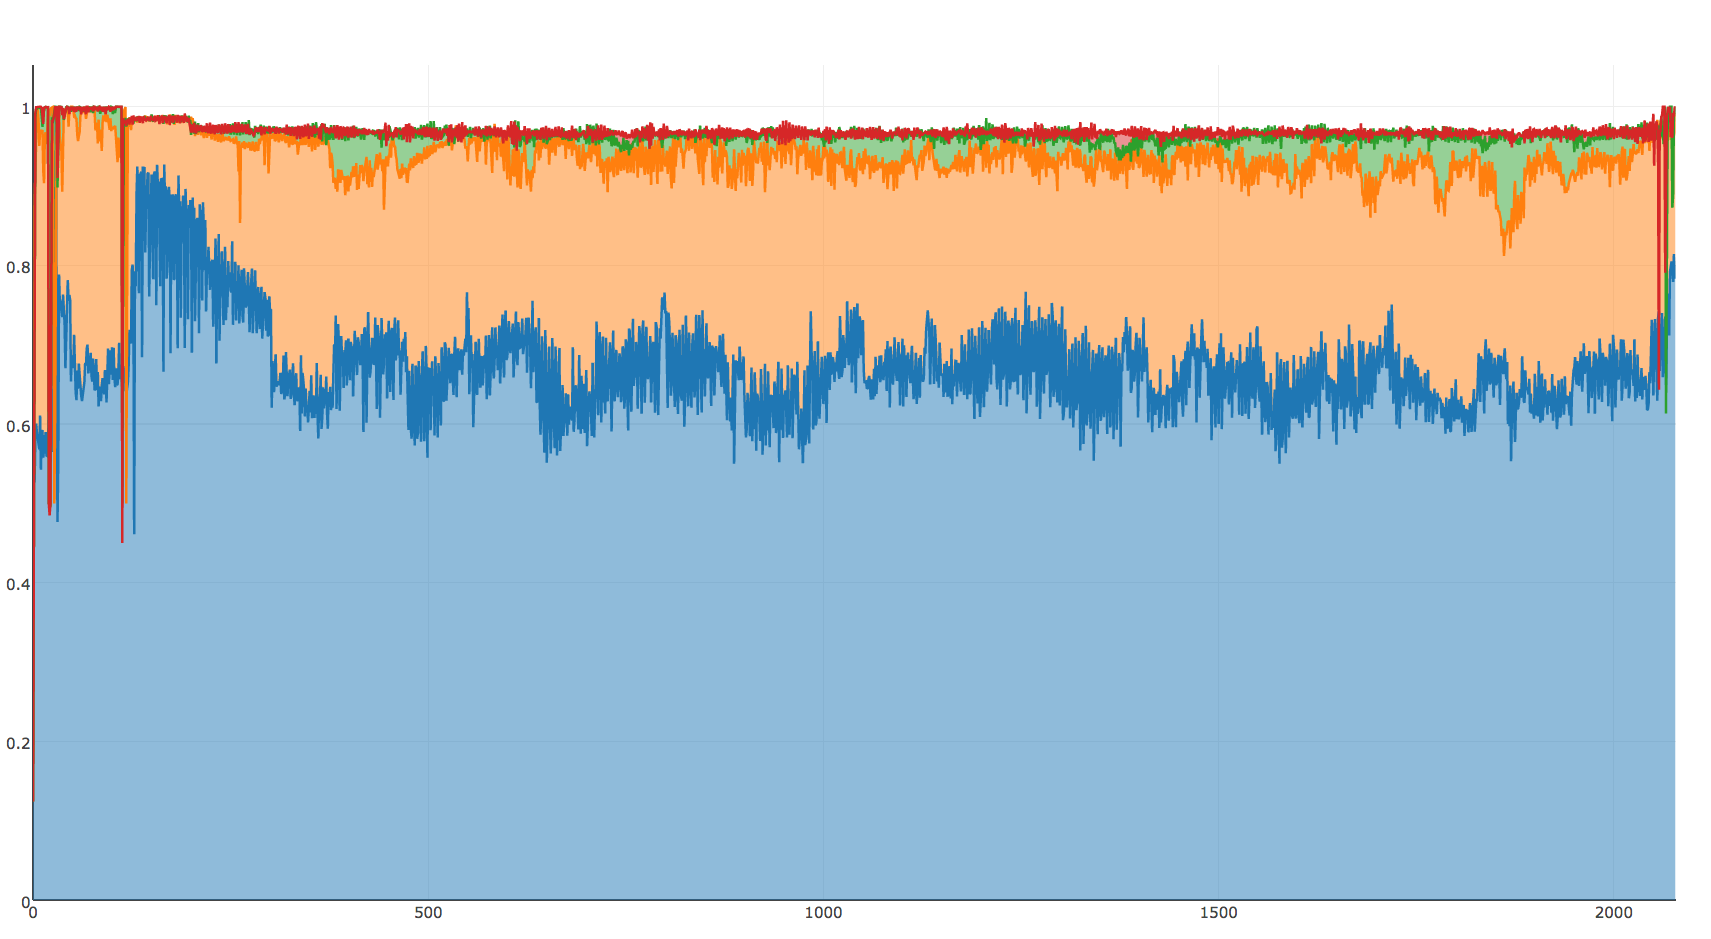
\includegraphics[width=\textwidth]{./pics/ispass_NN_all_windows}
\caption{%
روند رشد نرخ برخورد با افزایش اندازه حافظه نهان برای بارکاری
NN
از پکیج
ISPASS
}
\end{sidewaysfigure}

\begin{sidewaysfigure}
\centering
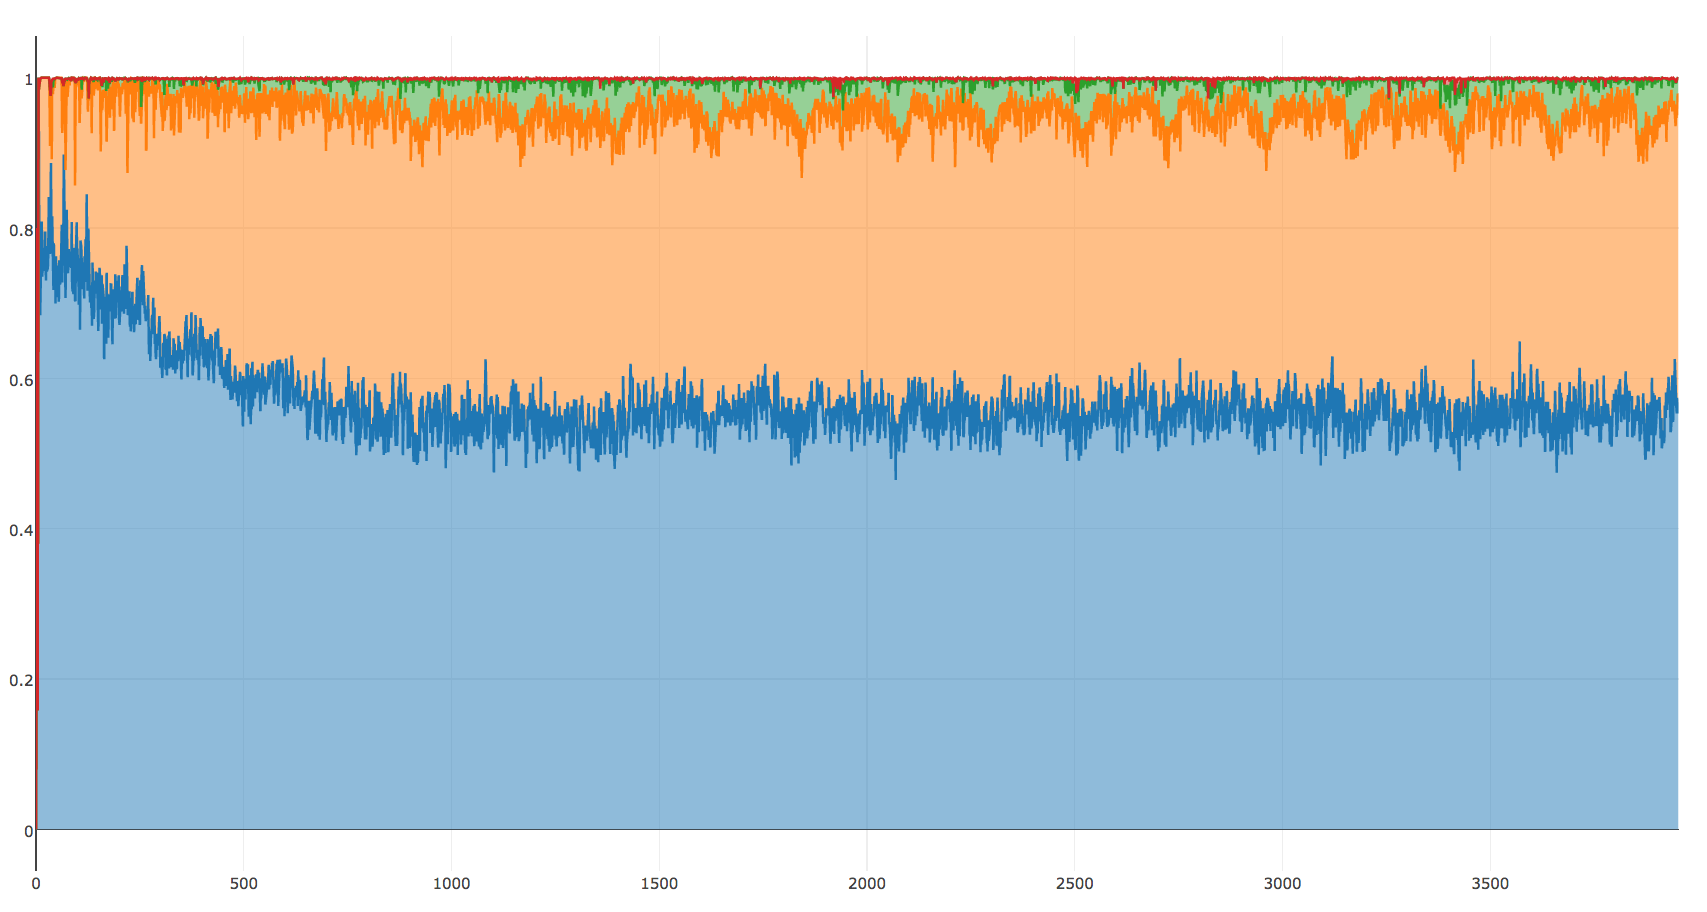
\includegraphics[width=\textwidth]{./pics/parboil_sad_all_windows}
\caption{%
روند رشد نرخ برخورد با افزایش اندازه حافظه نهان برای بارکاری
SAD
از پکیج
پاربویل
}
\end{sidewaysfigure}

\begin{sidewaysfigure}
\centering
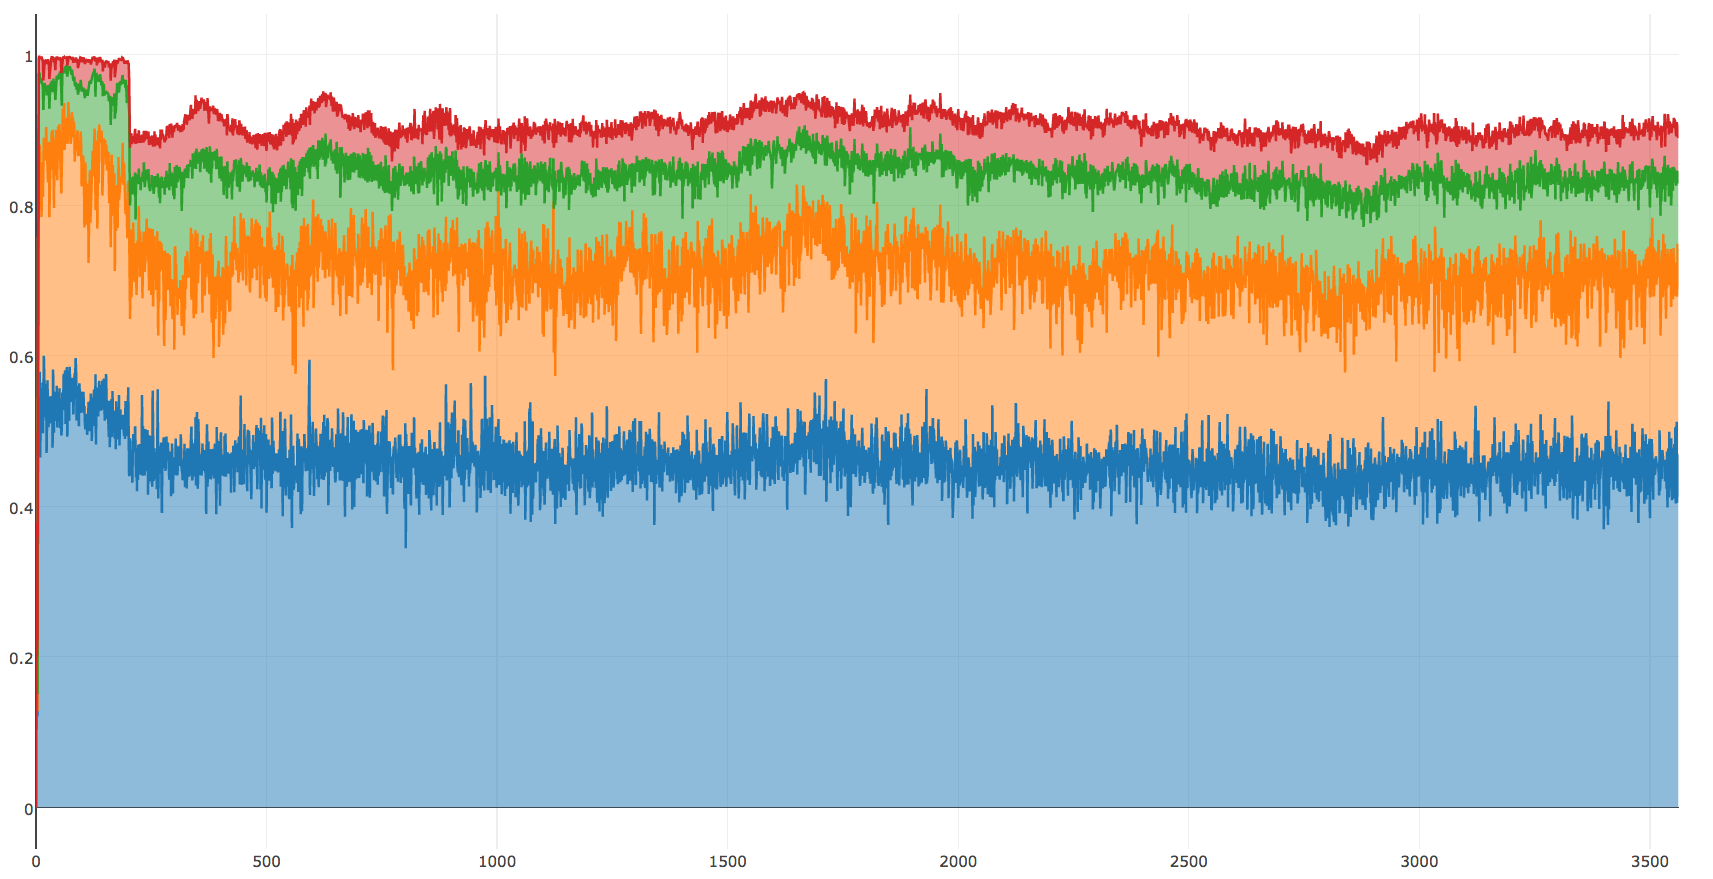
\includegraphics[width=\textwidth]{./pics/rodinia_leukocyte_all_windows}
\caption{%
روند رشد نرخ برخورد با افزایش اندازه حافظه نهان برای بارکاری
Leukocyte
از پکیج
رودینیا
}
\end{sidewaysfigure}

\section{
عملکرد حافظه نهان برای آدرس‌های حافظه مشترک
}

با توجه به حجم کم حافظه مشترک برای هر چندپردازنده به نظر می‌رسد که نیاز به در نظر گرفتن حافظه نهان چندان بزرگی برای آن نباشد. مشابه قسمت قبل  این‌بار فقط آدرس‌های مشترک را به شبیه‌ساز می‌دهیم و نتایج را ثبت می‌کنیم.

\begin{center}
\begin{table}[h!]
\begin{latin}
\begin{tabular}{|p{0.19\textwidth}|p{0.19\textwidth}|p{0.19\textwidth}|p{0.19\textwidth}|p{0.19\textwidth}|}
\hline
Workload/Cache Size & 16Kb  & 32Kb  & 48Kb  & 64Kb \\
\hline
LPS                 & 0.999695 & 0.999691 & 0.999693 & 0.999693 \\
\hline
NQU                 & 0.986432 & 0.987453 & 0.987623 & 0.988002 \\
\hline
STO                 & 0.999987 & 0.999982 & 0.999984 & 0.999991 \\
\hline
\end{tabular}
\end{latin}
\caption{%
\rl{%
درصد برخورد حافظه نهان برای آدرس‌های
مشترک
 بارهای کاری بنچمارک
ISPASS
}
}
\label{table:parboilhitrate}
\end{table}
\end{center}

\begin{center}
\begin{table}[h!]
\begin{latin}
\begin{tabular}{|p{0.19\textwidth}|p{0.19\textwidth}|p{0.19\textwidth}|p{0.19\textwidth}|p{0.19\textwidth}|}
\hline
Workload/Cache Size & 16Kb  & 32Kb  & 48Kb  & 64Kb \\
\hline
Heart Wall          & 0.999994 & 0.999997 & 0.999996 & 0.999990 \\
\hline
NW                  & 0.991531 & 0.991709 & 0.992185 & 0.992831 \\
\hline
Particle Filter     & 0.784459 & 0.806113 & 0.800006 & 0.827585 \\
\hline
\end{tabular}
\end{latin}
\caption{%
\rl{%
درصد برخورد حافظه نهان برای آدرس‌های
مشترک
 بارهای کاری بنچمارک
رودینیا
}
}
\label{table:parboilhitrate}
\end{table}
\end{center}

\begin{center}
\begin{table}[h!]
\begin{latin}
\begin{tabular}{|p{0.19\textwidth}|p{0.19\textwidth}|p{0.19\textwidth}|p{0.19\textwidth}|p{0.19\textwidth}|}
\hline
Workload/Cache Size & 16Kb  & 32Kb  & 48Kb  & 64Kb \\
\hline
BFS                 & 0.998965 & 0.999036 & 0.998903 & 0.999750 \\
\hline
MRI-GRIDDING        & 0.998132 & 0.998161 & 0.998178 & 0.998232 \\
\hline
\end{tabular}
\end{latin}
\caption{%
\rl{%
درصد برخورد حافظه نهان برای آدرس‌های
مشترک
 بارهای کاری بنچمارک
پاربویل
}
}
\label{table:parboilhitrate}
\end{table}
\end{center}

از آن‌جا که تمام اعداد نزدیک به یک هستند داده‌های با احتمال خطای زیاد حذف شده است. در هر صورت با توجه به اندازه کوچک حافظه نهان و نیز پیش بینی الگو‌های دسترسی به آن چنین نتایجی مورد انتظار است. همچنین می‌توان نتیجه‌گیری کرد که احتمالا با اندازه‌های حافظه نهان کوچکتر و یا استفاده از یک حافظه نهان نگاشت
\LTRfootnote{Direct Mapped Cache}
 مستقیم بتوان نتایج بهتری نیز گرفت. تحلیل دقیق این مورد نیازمند به دست آوردن داده‌های طول عمر آدرس‌ها در حافظه نهان است که جزو قدم‌های بعدی خواهد بود.
 
\subsection{
بررسی بهبود نرخ دستور در واحد زمان
}

یکی از معیار‌های اصلی برای سنجش بهبود عملکرد فاکتور
IPC
یا تعداد دستورالعمل اجرا شده در واحد زمان است. این کمیت توسط شبیه‌ساز
GPGPUSim
گزارش داده می‌شود و در نمودار‌های زیر میانگین‌آن برای تمام طول اجرای بارهای کاری مختلف را رسم شده است.

\begin{figure}[h]
\centering
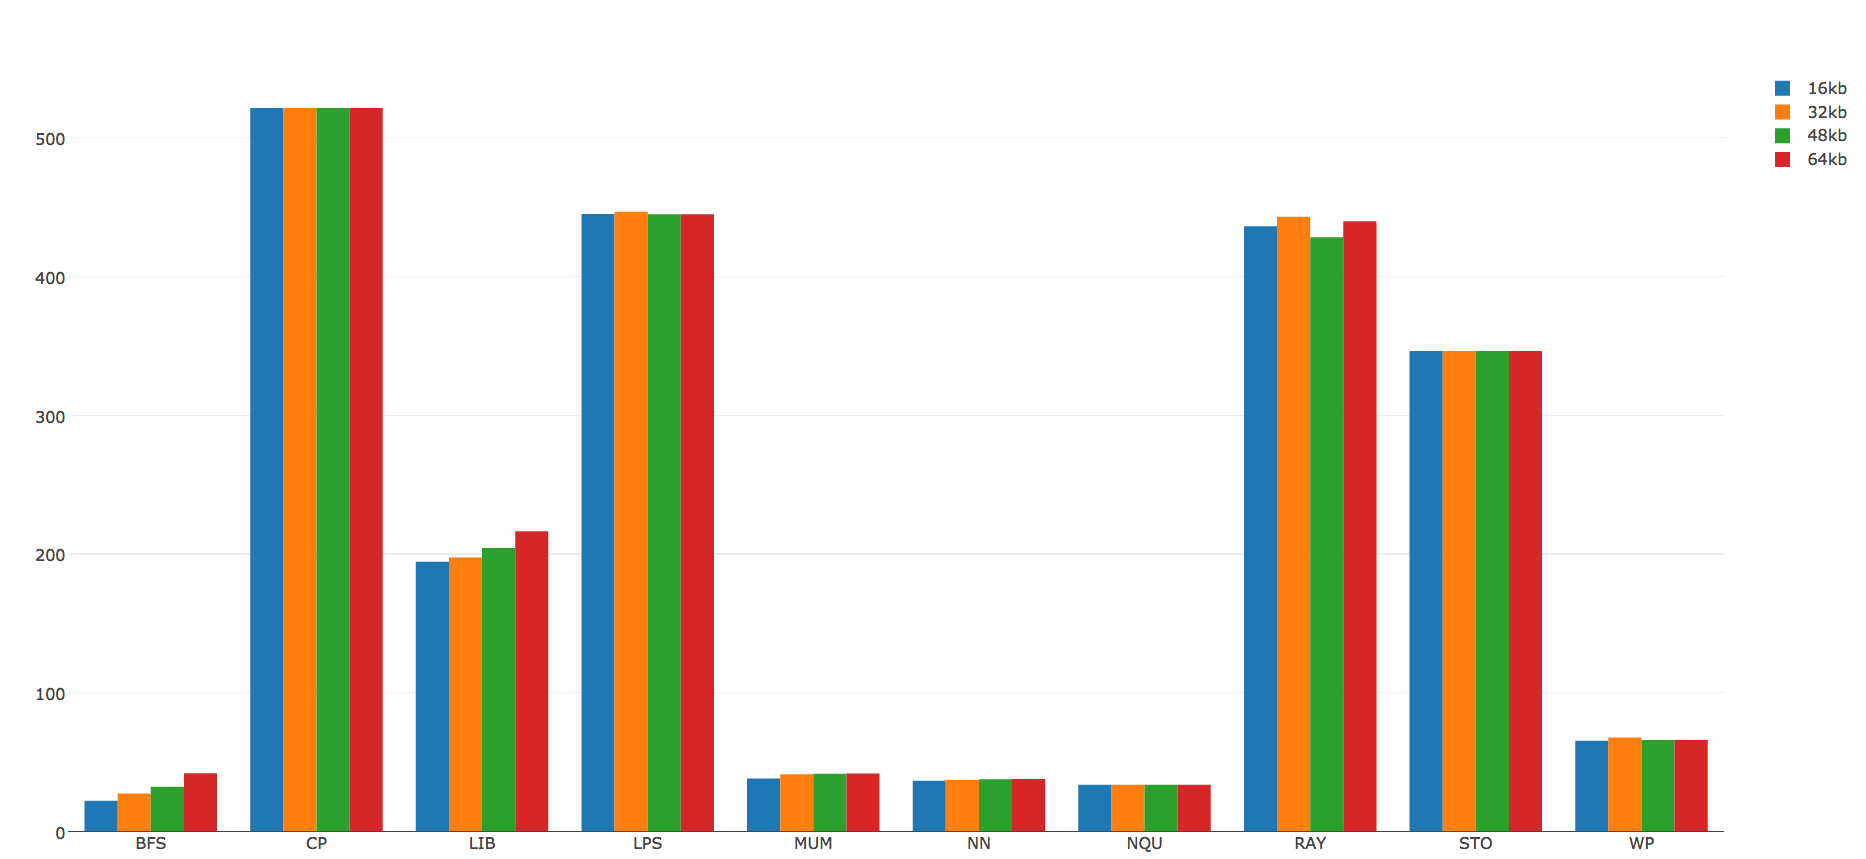
\includegraphics[width=\textwidth]{./pics/all_ipc_ispass}
\caption{
نرخ
IPC
برای اندازه‌های متفاوت حافظه نهان بنچمارک
ISPASS
}
\end{figure}

\begin{figure}[h]
\centering
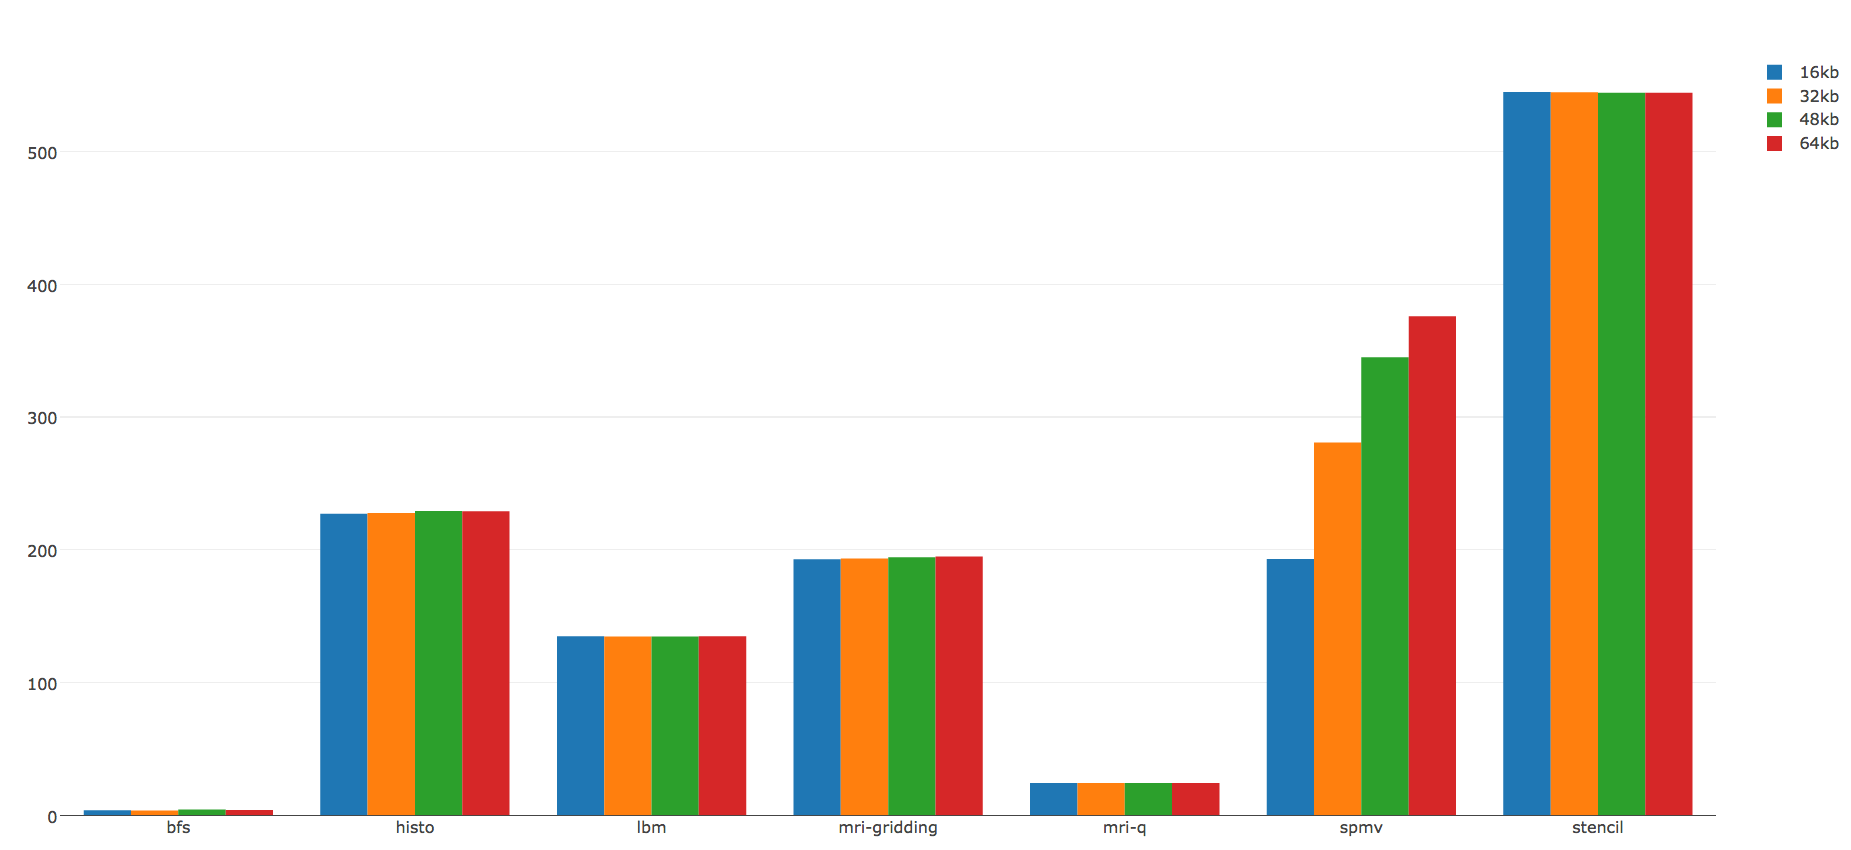
\includegraphics[width=\textwidth]{./pics/all_ipc_parboil}
\caption{
نرخ
IPC
برای اندازه‌های متفاوت حافظه نهان بنچمارک
پاربویل
}
\end{figure}


\begin{figure}[h]
\centering
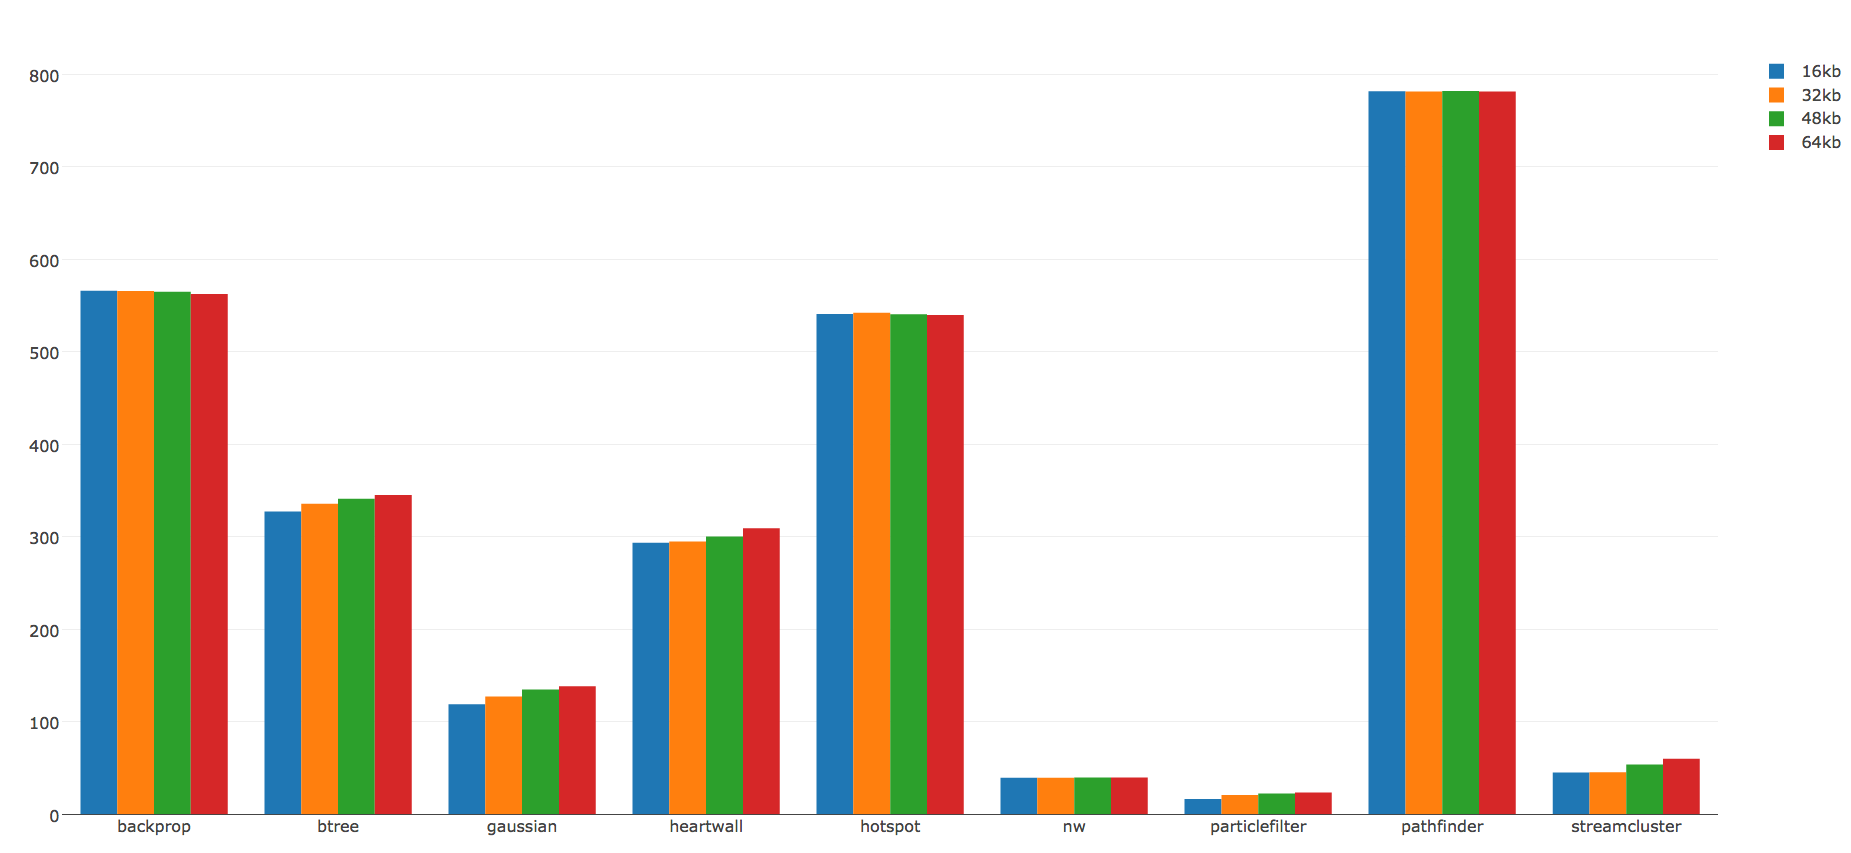
\includegraphics[width=\textwidth]{./pics/all_ipc_rodinia}
\caption{
نرخ
IPC
برای اندازه‌های متفاوت حافظه نهان بنچمارک
رودینیا
}
\end{figure}

این نمودار‌ها رشد پیوسته مقادیر 
IPC
با افزایش اندازه حافظه نهان را برای اکثر بارهای کاری نشان می‌دهند.
لازم به ذکر است در بعضی موارد ممکن است مقدار
IPC
به سبب عوامل دیگری مانند وابستگی داده‌ای بین ریسه‌ها و یا پهنا‌باند حافظه پردازنده میزبان محدود شده باشد که در این صورت نباید انتظار بهبودی به واسطه معماری پیشنهادی را داشت.

% Next %%%%%%%%%%%%%%%%%%%%%%%%%%%%%%%%%%%%%%%%%%%%%%%%%%%%%%%%%%%%%%%%%%%%%%%%%%%
\chapter{
جمع‌بندی و کار‌های آینده
}

امروزه پردازنده‌های گرافیکی عام‌منظوره به بستری محبوب برای پردازش‌های سریع تبدیل شده‌اند. رابط‌های نرم‌افزاری این پردازنده‌ها به برنامه‌نویسان این امکان را می‌دهند که پردازش‌های خود را در قالب هزاران ریسه که در گروه‌های کوچکتر که هر یک دستور ثابتی را اجرا می‌کنند دسته‌بندی‌ شده‌اند مدل‌سازی کنند. کارهای پیشین نشان داده‌ است که این رویکرد سبب افزایش چندین مرتبه‌ای سرعت برای برخی پردازش‌ها می‌شود.

یکی از عواملی که عملکرد پردازنده‌های گرافیکی را محدود می‌کند استفاده نامناسب
\LTRfootnote{Underutilization}
از حافظه مشترک چند‌پردازنده‌هاست. این امر می‌تواند به علت نیاز به دسترسی ریسه‌ها به داده‌های مشترک از حافظه چرک‌نویس و وابستگی‌داده‌ای و بین‌ آن‌ها و در موارد کمبود پهنای باند این حافظه سبب محدودیت اجرای ریسه‌ها و به تبع آن کاهش
\textit{
موازات سطح ریسه
}
\LTRfootnote{Thread Level Parallelism (TLP)}
شود. این امر به خصوص در بارهای کاری با محاسبات سنگین می‌تواند کاهش عملکرد پردازنده شود. مطالعات قبلی در این حوزه نشان داده است که پهنای باند حافظه اصلی معمولا بسیار بیشتر از حد مورد نیاز در بارهای پردازشی است. با تکیه بر این دانسته می‌توان امیدوار بود که انتقال ترافیک حافظه مشترک به درگاه
DRAM
سبب بهبود نرخ
TLP
شود.

برای استفاده حداکثری از موازات گسترده فراهم شده توسط پردازنده‌های گرافیکی نیاز است تا داده‌های مورد نیاز هر هسته پردازشی در زمان کوتاهی برای آن قابل دسترسی باشد و  عملکرد مناسب حافظه نهان می‌تواند در اینجا بسیار حیاتی باشد.
تا به اینجای کار نشان داده‌ایم که افزایش حجم حافظه نهان به یقین تاثیر مثبت قابل توجهی رو نرخ برخورد و نیز مقادیر
IPC
برای بارهای کاری عام‌منظوره داشته باشد. همچنین می‌بینیم که اختصاص قسمت کوچکی از حافظه نهان هر چندپردازنده به فضای آدرس مشترک می‌تواند تضمین‌کننده نرخ برخورد بالا باشد. این مشاهدات شهود اولیه ما را تایید می‌کند ولی همچنان نیاز به 
بررسی دقیق‌تر برای امکان‌سنجی پیاده‌سازی این معماری وجود دارد.

در نظر داشته باشیم که تا به اینجای کار هنوز تاثیر تاخیر ایجاد شده به واسطه انتقال داده‌های فضای مشترک به حافظه اصلی را در نظر گرفته نشده است. همچنین تاثیر بار اضافه شده بر درگاه حافظه
DRAM
بر عملکرد سایر قسمت‌های پردازنده نیز باید به نوعی در نتیجه‌گیری لحاظ شود. از مواردی که می‌تواند در ادامه‌ی این پروژه قرار بگیرد اعمال تغییرات لازم در شبیه‌ساز به منظور نگاشت فضای آدرس‌دهی مشترک به حافظه اصلی است. همچنین با تحلیل دقیق‌تر الگوی دسترسی به حافظه‌نهان و حافظه مشترک و نیز اضافه کردن بارهای کاری جدید به مجموعه فعلی می‌توان یک الگوریتم واکشی ‌پیش‌دستانه
\LTRfootnote{Pre-Fetching}
طراحی کرد تا عملکرد حافظه نهان را به خصوص در هنگام بازگرداندن داده‌های قدیمی به حافظه اصلی بهبود بخشید.


% Bibliography %%%%%%%%%%%%%%%%%%%%%%%%%%%%%%%%%%%%%%%%%%%
\PrepareForBiblio
\begin{thebibliography}{1}
\begin{LTRitems}

\setpersianfont\bibitem{cite1}\resetlatinfont
\newblock S. Borkar, {\itshape``Design challenges of technology scaling''} in
IEEE Micro,
vol.
19,
no. 4, pp. 23-29, Jul-Aug 1999.

\setpersianfont\bibitem{cite2}\resetlatinfont
\newblock M. D. Hill and M. R. Marty, {\itshape``Amdahl's Law in the Multicore
Era,''} in
Computer,
vol. 41, no. 7, pp. 33-38, July 2008.

\setpersianfont\bibitem{cite3}\resetlatinfont
\newblock Nvidia Corportaion, {\itshape``
\href{https://www.nvidia.com/content/PDF/kepler/NVIDIA-Kepler
-GK110-Architecture-Whitepaper.pdf}{Nvidia Kepler GK110 Architecture
Whitepaper}}''

\setpersianfont\bibitem{cite4}\resetlatinfont
\newblock R. H. Dennard, F. H. Gaensslen, V. L. Rideout, E. Bassous and A. R.
LeBlanc, {\itshape``Design of ion-implanted MOSFET's with very small physical
dimensions,''} in IEEE Journal of Solid-State Circuits, vol. 9, no. 5, pp.
256-268, Oct 1974.

\setpersianfont\bibitem{cite5}\resetlatinfont
\newblock D. Luebke, {\itshape ``CUDA: Scalable parallel programming for
high-performance
scientific
computing''}, 2008 5th IEEE International Symposium on Biomedical Imaging: From
Nano to Macro, Paris, 2008, pp. 836-838.

\setpersianfont\bibitem{cite6}\resetlatinfont
\newblock Tyler Sorensen, Ganesh Gopalakrishnan, and Vinod Grover. 2013.
{\itshape ``Towards
shared
memory consistency models for GPUs''}. In Proceedings of the 27th international
ACM conference on International conference on supercomputing (ICS '13)

\setpersianfont\bibitem{cite7}\resetlatinfont
\newblock A. Bakhoda, G. L. Yuan, W. W. L. Fung, H. Wong and T. M. Aamodt,
{\itshape ``Analyzing
CUDA workloads using a detailed GPU simulator," 2009 IEEE International
Symposium on Performance Analysis of Systems and Software, Boston''}, MA, 2009,
pp. 163-174.

\setpersianfont\bibitem{cite8}\resetlatinfont
\newblock S. Che et al., {\itshape ``Rodinia: A benchmark suite for
heterogeneous
computing,''} 2009
IEEE International Symposium on Workload Characterization (IISWC), Austin, TX,
2009, pp. 44-54.

\setpersianfont\bibitem{cite9}\resetlatinfont
\newblock Che, Shuai, Jeremy W. Sheaffer, Michael Boyer, Lukasz G. Szafaryn,
Liang Wang, and Kevin Skadron. {\itshape ``A characterization of the Rodinia
benchmark
suite with comparison to contemporary CMP workloads.''} In Workload
Characterization (IISWC), 2010 IEEE International Symposium on, pp. 1-11. IEEE,
2010.

\setpersianfont\bibitem{cite10}\resetlatinfont
\newblock Stratton, John A., et al. {\itshape ``Parboil: A revised benchmark
suite
for
scientific
and commercial throughput computing.''} Center for Reliable and
High-Performance
Computing 127 (2012).

\setpersianfont\bibitem{cite11}\resetlatinfont
\newblock Kayıran, O., Jog, A., Kandemir, M.T. and Das, C.R., 2013, October.
{\itshape ``Neither more nor less: optimizing thread-level parallelism for GPGPUs''}. In Proceedings of the
22nd international conference on Parallel architectures and compilation
techniques (pp. 157-166). IEEE Press.

\setpersianfont\bibitem{cite12}\resetlatinfont
\newblock Jatala, Vishwesh, Jayvant Anantpur, and Amey Karkare.
{\itshape ``Scratchpad sharing in GPUs.''} arXiv preprint arXiv:1607.03238 (2016).

\setpersianfont\bibitem{cite13}\resetlatinfont
\newblock van den Braak, G.J., Gómez-Luna, J., Corporaal, H., Gonzalez-Linares, J.M. and Guil, N., 2013, October. {\itshape ``Simulation and architecture improvements of atomic operations on GPU scratchpad memory''}. In Computer Design (ICCD), 2013 IEEE 31st International Conference on (pp. 357-362). IEEE.

\setpersianfont\bibitem{cite14}\resetlatinfont
\newblock Puzak, Thomas Roberts. {\itshape ``Analysis of cache replacement-algorithms.''} (1985).

\setpersianfont\bibitem{cite15}\resetlatinfont
\newblock Gao, Shuang, and Gregory D. Peterson. {\itshape ``Optimizing CUDA Shared Memory Usage.''}

\setpersianfont\bibitem{cite15}\resetlatinfont
\newblock Glaskowsky, Peter N. {\itshape ``NVIDIA’s Fermi: the first complete GPU computing architecture.''} White paper 18 (2009).

\end{LTRitems}
\end{thebibliography}
%%%%%%%%%%%%%%%%%%%%%%%%%%%%%%%%%%%%%%%%%%%%%%%%%%%%%%%%%%
%%%%%%%%%%%%%%%%%%%%%%%%%%%%%%%%%%%%%%%%%%%%%%%%%%%%%%%%%%
%%%%%%%%%%%%%%%%%%%%%%%%%%%%%%%%%%%%%%%%%%%%%%%%%%%%%%%%%%
\PrepareForLatinPages
\date{June 25, 2017}
\title{\sffamily A Study on Performance of Shared Memory in GPGPUs}
\author{\sffamily Parsoa Khorsand RahimZadeh}
\university{Sharif University of Technology\\Department of Computer Engineering}
\subject{Software Engineering}
\supervisor{\sffamily Dr. Hamid Sarbazi Azad}
%%%%%%%%%%%%%%%%%%%%%%%%%%%%%%%%%%%%%%%%%%%%%%%%%%%%%%%%%%
\begin{abstract}{General Purpose Graphics Processing Unit, GPGPU, GPGPU-Sim, shared Memory, Scratchpad, Performance, TLP, IPC}
\end{
}
\makethesistitle
%%%%%%%%%%%%%%%%%%%%%%%%%%%%%%%%%%%%%%%%%%%%%%%%%%%%%%%%%%
\end{document}